\section{Coordinate systems}


\subsection{General 3D coordinate system}
\label{Sec2:general3DcoordinateSystem}
We shall now consider the general 3D coordinate system, which one may reduce to the the cylindrical coordinate system and the spherical coordinate system. Let the coordinate system be defined by
\begin{equation*}
	\vec{r} = \begin{bmatrix}
	x(\xi, \eta, \zeta)\\
	y(\xi, \eta, \zeta)\\
	z(\xi, \eta, \zeta)
\end{bmatrix} :	 \R^3\to\R^3, \quad  \begin{bmatrix}
	\xi\\
	\eta\\
	\zeta
	\end{bmatrix}\mapsto \vec{r}(\xi, \eta, \zeta).
\end{equation*}
We shall frequently use the scaling lengths defined by
\begin{align}
	h_{\upxi} &= \norm{\pderiv{\vec{r}}{\xi}} = \sqrt{\left(\pderiv{x}{\xi}\right)^2+\left(\pderiv{y}{\xi}\right)^2+\left(\pderiv{z}{\xi}\right)^2}\nonumber\\
	h_{\upeta} &= \norm{\pderiv{\vec{r}}{\eta}} = \sqrt{\left(\pderiv{x}{\eta}\right)^2+\left(\pderiv{y}{\eta}\right)^2+\left(\pderiv{z}{\eta}\right)^2}\label{Eq2:ScalingLengths}\\
	h_{\upzeta} &= \norm{\pderiv{\vec{r}}{\zeta}} = \sqrt{\left(\pderiv{x}{\zeta}\right)^2+\left(\pderiv{y}{\zeta}\right)^2+\left(\pderiv{z}{\zeta}\right)^2}.\nonumber
\end{align}
The standard basis vectors in this general coordinate system are then
\begin{equation*}
	\vec{e}_{\upxi} = \frac{1}{h_{\upxi}}\pderiv{\vec{r}}{\xi},\quad\vec{e}_{\upeta} = \frac{1}{h_{\upeta}}\pderiv{\vec{r}}{\eta},\quad\vec{e}_{\upzeta} = \frac{1}{h_{\upzeta}}\pderiv{\vec{r}}{\zeta}.
\end{equation*}
We now want to develop an expression for the nabla operator in terms of these unit vectors. In our coordinate system, the nabla operator is defined by
\begin{equation*}
	\nabla f = \vec{e}_{\upxi} g_{\upxi} +\vec{e}_{\upeta} g_{\upeta} +\vec{e}_{\upzeta} g_{\upzeta}.
\end{equation*}
where $g_{\upxi}$, $g_{\upeta}$ and $g_{\upzeta}$ are functionals of $f$ which are to be determined.

Moreover, the nabla operator satisfy
\begin{equation*}
	\diff f = \nabla f\cdot\diff \vec{r},
\end{equation*}
where (by the chain rule)
\begin{align*}
	\diff \vec{r} &= \pderiv{\vec{r}}{\xi}\diff\xi + \pderiv{\vec{r}}{\eta}\diff\eta + \pderiv{\vec{r}}{\zeta}\diff\zeta\\
	  &= h_{\upxi}\vec{e}_{\upxi} \diff\xi + h_{\upeta}\vec{e}_{\upeta} \diff\eta + h_{\upzeta}\vec{e}_{\upzeta} \diff\zeta.
\end{align*}
Using the chain rule once again, we also have
\begin{equation*}
	\diff f = \pderiv{f}{\xi} \diff\xi + \pderiv{f}{\eta} \diff\eta + \pderiv{f}{\zeta} \diff\zeta.
\end{equation*}
Combining the equations for $\diff f$ we get the relation
\begin{align}
	\pderiv{f}{\xi} \diff\xi + \pderiv{f}{\eta} \diff\eta + \pderiv{f}{\zeta} \diff\zeta &= \left(\vec{e}_{\upxi} g_{\upxi} +\vec{e}_{\upeta} g_{\upeta} +\vec{e}_{\upzeta} g_{\upzeta}\right)\cdot\left(h_{\upxi}\vec{e}_{\upxi} \diff\xi + h_{\upeta}\vec{e}_{\upeta} \diff\eta + h_{\upzeta}\vec{e}_{\upzeta} \diff\zeta\right)\\
	&=h_{\upxi}(g_{\upxi} +  \vec{e}_{\upxi}\cdot \vec{e}_{\upeta} g_{\upeta} +  \vec{e}_{\upxi}\cdot\vec{e}_{\upzeta} g_{\upzeta})\diff\xi\\
	&+h_{\upeta}(\vec{e}_{\upxi}\cdot \vec{e}_{\upeta} g_{\upxi} +  g_{\upeta} +  \vec{e}_{\upeta}\cdot\vec{e}_{\upzeta} g_{\upzeta})\diff\eta\\
	&+h_{\upzeta}(\vec{e}_{\upxi}\cdot \vec{e}_{\upzeta} g_{\upxi} +  \vec{e}_{\upeta}\cdot\vec{e}_{\upzeta} g_{\upeta}+  g_{\upzeta})\diff\zeta
\end{align}
where we have used the fact that $\vec{e}_{\upxi}\cdot\vec{e}_{\upxi}= 1$, $\vec{e}_{\upeta}\cdot\vec{e}_{\upeta}= 1$ and $\vec{e}_{\upzeta}\cdot\vec{e}_{\upzeta}= 1$. As the coefficients in front of $\diff\xi$, $\diff\eta$ and $\diff\zeta$ must be the same on both side, we get a system of equations given by
\begin{equation}\label{Eq2:systemNablaOperator}
\begin{alignedat}{4}
	 g_{\upxi} & {}+{} &  \vec{e}_{\upxi}\cdot \vec{e}_{\upeta} g_{\upeta} & {}+{} &  \vec{e}_{\upxi}\cdot\vec{e}_{\upzeta} g_{\upzeta} &= \frac{1}{h_{\upxi}}\pderiv{f}{\xi}\\
	\vec{e}_{\upxi}\cdot \vec{e}_{\upeta} g_{\upxi} & {}+{} &  g_{\upeta} & {}+{} & \vec{e}_{\upeta}\cdot\vec{e}_{\upzeta} g_{\upzeta} &= \frac{1}{h_{\upeta}}\pderiv{f}{\eta}\\
	\vec{e}_{\upxi}\cdot \vec{e}_{\upzeta} g_{\upxi} & {}+{} & \vec{e}_{\upeta}\cdot\vec{e}_{\upzeta} g_{\upeta} & {}+{} & g_{\upzeta} &= \frac{1}{h_{\upzeta}}\pderiv{f}{\zeta}.
\end{alignedat}
\end{equation}
Introducing the notation
\begin{equation*}
	E_{\upxi\upeta} = \vec{e}_{\upxi}\cdot\vec{e}_{\upeta},\quad E_{\upxi\upzeta} = \vec{e}_{\upxi}\cdot\vec{e}_{\upzeta},\quad E_{\upeta\upzeta} = \vec{e}_{\upeta}\cdot\vec{e}_{\upzeta}
\end{equation*}
the system in \Cref{Eq2:systemNablaOperator} is given by can be written as
\begin{equation*}
	\begin{bmatrix}
		1 & E_{\upxi\upeta} & E_{\upxi\upzeta}\\
		E_{\upxi\upeta} & 1 & E_{\upeta\upzeta}\\
		E_{\upxi\upzeta} & E_{\upeta\upzeta} & 1\\
	\end{bmatrix}\begin{bmatrix}
		g_{\upxi}\\
		g_{\upeta}\\
		g_{\upzeta}
	\end{bmatrix} = \begin{bmatrix}
	\frac{1}{h_{\upxi}} \pderiv{f}{\xi}\\
	\frac{1}{h_{\upeta}} \pderiv{f}{\eta}\\
	\frac{1}{h_{\upzeta}} \pderiv{f}{\zeta}\end{bmatrix}.
\end{equation*}
As the determinant of this system of equation is given by
\begin{equation*}
	\nabla^2 = 1 - E_{\upxi\upeta}^2 - E_{\upxi\upzeta}^2 - E_{\upeta\upzeta}^2 + 2E_{\upxi\upeta}E_{\upxi\upzeta}E_{\upeta\upzeta}
\end{equation*}
we may write the solution as
\begin{align*}
\begin{bmatrix}
	g_{\upxi}\\
	g_{\upeta}\\
	g_{\upzeta}
\end{bmatrix} = \begin{bmatrix}
	a_{11} & a_{12} & a_{13}\\
	a_{21} & a_{22} & a_{23}\\
	a_{31} & a_{32} & a_{33}
\end{bmatrix} \begin{bmatrix}
	\frac{1}{h_{\upxi}} \pderiv{f}{\xi}\\
	\frac{1}{h_{\upeta}} \pderiv{f}{\eta}\\
	\frac{1}{h_{\upzeta}} \pderiv{f}{\zeta}
\end{bmatrix}
\end{align*}
where the coefficients $a_{ij}$ are given by the symmetric matrix
\begin{equation*}
	[a_{ij}] = \frac{1}{\nabla^2}\begin{bmatrix}
		1-E_{\upeta\upzeta}^2 & E_{\upxi\upzeta}E_{\upeta\upzeta} - E_{\upxi\upeta}  &  E_{\upxi\upeta}E_{\upeta\upzeta} - E_{\upxi\upzeta}\\
		E_{\upxi\upzeta}E_{\upeta\upzeta} - E_{\upxi\upeta} & 1-E_{\upxi\upzeta}^2 & E_{\upxi\upeta}E_{\upxi\upzeta} - E_{\upeta\upzeta}\\
		E_{\upxi\upeta}E_{\upeta\upzeta} - E_{\upxi\upzeta} & E_{\upxi\upeta}E_{\upxi\upzeta} - E_{\upeta\upzeta} & 1-E_{\upxi\upeta}^2
	\end{bmatrix}
\end{equation*}
Let's verify this calculation by finding the nabla operator in the spherical coordinate system. Letting $\xi$ correspond to the azimuthal angle $\phi$, $\eta$ the polar angle $\vartheta$ and $\zeta$ the radial direction $r$, we have the relations
\begin{align*}
	x &= \zeta\sin\eta\cos\xi\\
	y &= \zeta\sin\eta\sin\xi\\
	z &= \zeta\cos\eta.
\end{align*}
As the spherical coordinate system is an orthogonal coordinate system, we get $E_{\upxi\upeta}=0$, $E_{\upxi\upzeta}=0$ and $E_{\upeta\upzeta}=0$. Thus,
\begin{equation*}
	g_{\upxi} = \frac{1}{h_{\upxi}}\pderiv{f}{\xi},\quad g_{\upeta} =\frac{1}{h_{\upeta}}\pderiv{f}{\eta},\quad g_{\upzeta} =\frac{1}{h_{\upzeta}}\pderiv{f}{\zeta}.
\end{equation*}
By computation, we find
\begin{equation*}
	h_{\upxi} = \zeta\sin\eta,\quad h_{\upeta} = \zeta,\quad h_{\upzeta} = 1.
\end{equation*}
Thus,
\begin{align*}
	\nabla f &= \frac{1}{\zeta\sin\eta}\pderiv{f}{\xi}\vec{e}_{\upxi} + \frac{1}{\zeta}\pderiv{f}{\eta}\vec{e}_{\upeta} + \pderiv{f}{\zeta}\vec{e}_{\upzeta}\\
	&= \pderiv{f}{r}\vec{e}_{\mathrm{r}} + \frac{1}{r}\pderiv{f}{\vartheta}\vec{e}_{\upvartheta} + \frac{1}{r\sin\vartheta}\pderiv{f}{\phi}\vec{e}_{\upphi},
\end{align*}
which is the familiar expression for the nabla operator in spherical coordinates.

\subsubsection{Extended NURBS coordinate system}
\label{subsubsubsec:infElementsOnGeneralizedCoordSyst}
In this section we shall explore the possibility to have a more general coordinate system for the infinite elements. All though the prolate spheroidal coordinate system helps reduce the number of elements needed to circumference a long obstacle compared to the spherical coordinate system, it is still not ideal with respect to this problem. It is possible to define a coordinate system such that we get
\begin{equation*}
	\inf_{\vec{x}\in\Gamma} \| \vec{x} - \vec{y}_0 \| = \inf_{\vec{y}\in\Gamma_{\mathrm{a}}} \| \vec{x}_0-\vec{y}\|\quad \forall\vec{x}_0\in\Gamma,\quad\text{and}\quad\forall\vec{y}_0\in\Gamma_{\mathrm{a}}.
\end{equation*}
That is, we can have the surface $\Gamma_{\mathrm{a}}$ at a constant distance from the surface $\Gamma$ (if $\Gamma$ is convex\footnote{If this is not the case, an intermediate convex surface must be inserted between $\Gamma$ and $\Gamma_{\mathrm{a}}$ in the NURBS patch.}). However, is it possible to define a infinite element formulation on such a coordinate system? The most intuitive coordinate system would satisfy the property that for all points on $\Gamma_{\mathrm{a}}$ the normal vector is parallel to the ``radial'' unit vector for this coordinate system. This would however make the integration in the weak formulation hard as the nabla operator would not be separable, and we may no longer integrate analytically in the ``radial'' direction. In the following we shall consider another option which results in a separable nabla operator.

Let's build upon the theory developed in \Cref{Sec2:general3DcoordinateSystem} where we shall assume that the NURBS parametrization at hand has a ``radial'' parameter $\zeta$, such that $\xi$ and $\eta$ corresponds to ``angular'' parameters. This will typically be the case when considering shell objects, where $\zeta$ will run through the thickness of the elastic material. We know that at any given value $\bar{\zeta}$ the NURBS solid in 3D reduces to a NURBS surface in 3D. This is in particular true for $\bar{\zeta} = 1$, which will be our artificial boundary $\Gamma_{\mathrm{a}}$. We shall assume, without loss of generality, that the NURBS surface $\Gamma_{\mathrm{a}}$ fully encloses the origin. Finally, we assume the surface $\Gamma_{\mathrm{a}}$ to be a convex surface. We now want to extend the NURBS parametrization also for $\zeta > 1$. In particular we define (for $\zeta>1$)
\begin{equation*}
	\vec{r} = \begin{bmatrix}
	x(\xi, \eta, \zeta)\\
	y(\xi, \eta, \zeta)\\
	z(\xi, \eta, \zeta)
\end{bmatrix} :	 \R^3\to\R^3, \quad  \begin{bmatrix}
	\xi\\
	\eta\\
	\zeta
	\end{bmatrix}\mapsto s(\zeta)\bar{\vec{r}}(\xi, \eta).
\end{equation*}
where $\bar{\vec{r}}$ is the NURBS 3D surface at $\zeta = 1$ and the \textit{scaling function} $s$ is strictly increasing and satisfies $s(1) = 1$. Thus, for any $\zeta > 1$ we simply get a scaled version of $\Gamma_{\mathrm{a}}$ from the origin with the scaling factor $s(\zeta)$.

Continuing on the notation from \Cref{Sec2:general3DcoordinateSystem}, our new coordinate system has the following nice property
\begin{equation*}
	h_{\upxi} = s(\zeta)\norm{\pderiv{\bar{\vec{r}}}{\xi}},\quad h_{\upeta} = s(\zeta)\norm{\pderiv{\bar{\vec{r}}}{\eta}},\quad h_{\upzeta} = s'(\zeta)\norm{\bar{\vec{r}}}.
\end{equation*}
From this we observe that the unit vectors $\vec{e}_{\upxi}$, $\vec{e}_{\upeta}$ and $\vec{e}_{\upzeta}$ are all independent of $\zeta$. Moreover, $E_{\upxi\upeta}$, $E_{\upxi\upzeta}$ and $E_{\upeta\upzeta}$ (and thus also the determinant $\nabla^2$) will also be independent of $\zeta$. The resulting nabla operator will then be separable, which we will take advantage of. In this context we define 
\begin{equation*}
	\bar{h}_{\upxi} = \norm{\pderiv{\bar{\vec{r}}}{\xi}}, \quad \bar{h}_{\upeta} = \norm{\pderiv{\bar{\vec{r}}}{\eta}},\quad \bar{h}_{\upzeta} = \norm{\bar{\vec{r}}}
\end{equation*}
such that $h_{\upxi} = s(\zeta)\bar{h}_{\upxi}$, $h_{\upeta} = s(\zeta)\bar{h}_{\upeta}$, $h_{\upzeta} = s'(\zeta)\bar{h}_{\upzeta}$. We may now easy see that the nabla operator is separable as it is now given by (for $\zeta>1$)
\begin{align*}
	\nabla &= \left(\frac{a_{11}}{s(\zeta)\bar{h}_{\upxi}}\pderiv{}{\xi} + \frac{a_{12}}{s(\zeta)\bar{h}_{\upeta}}\pderiv{}{\eta} + \frac{a_{13}}{s'(\zeta)\bar{h}_{\upzeta}}\pderiv{}{\zeta}\right)\vec{e}_{\upxi}\\
	 &+\left(\frac{a_{21}}{s(\zeta)\bar{h}_{\upxi}}\pderiv{}{\xi} + \frac{a_{22}}{s(\zeta)\bar{h}_{\upeta}}\pderiv{}{\eta} + \frac{a_{23}}{s'(\zeta)\bar{h}_{\upzeta}}\pderiv{}{\zeta}\right)\vec{e}_{\upeta}\\
	 &+ \left(\frac{a_{31}}{s(\zeta)\bar{h}_{\upxi}}\pderiv{}{\xi} + \frac{a_{32}}{s(\zeta)\bar{h}_{\upeta}}\pderiv{}{\eta} + \frac{a_{33}}{s'(\zeta)\bar{h}_{\upzeta}}\pderiv{}{\zeta}\right)\vec{e}_{\upzeta}\\
	 &= \frac{1}{s(\zeta) \bar{h}_{\upxi}}\left(a_{11}\vec{e}_{\upxi} + a_{21} \vec{e}_{\upeta} + a_{31}\vec{e}_{\upzeta}\right)\pderiv{}{\xi}\\
	 &+\frac{1}{s(\zeta)\bar{h}_{\upeta}}\left(a_{12}\vec{e}_{\upxi} + a_{22} \vec{e}_{\upeta} + a_{32}\vec{e}_{\upzeta}\right)\pderiv{}{\eta}\\
	 &+\frac{1}{s'(\zeta)\bar{h}_{\upzeta}}\left(a_{13}\vec{e}_{\upxi} + a_{23} \vec{e}_{\upeta} + a_{33}\vec{e}_{\upzeta}\right)\pderiv{}{\zeta}\\
	 &= \frac{1}{s(\zeta)}\nabla_S + \frac{1}{s'(\zeta)}\vec{a}\pderiv{}{\zeta}
\end{align*}
where
\begin{equation*}
	\nabla_S = \frac{1}{\bar{h}_{\upxi}}\left(a_{11}\vec{e}_{\upxi} + a_{21} \vec{e}_{\upeta} + a_{31}\vec{e}_{\upzeta}\right)\pderiv{}{\xi}+\frac{1}{\bar{h}_{\upeta}}\left(a_{12}\vec{e}_{\upxi} + a_{22} \vec{e}_{\upeta} + a_{32}\vec{e}_{\upzeta}\right)\pderiv{}{\eta}
\end{equation*}
and
\begin{equation*}
	\vec{a} = \frac{1}{\bar{h}_{\upzeta}}\left(a_{13}\vec{e}_{\upxi} + a_{23} \vec{e}_{\upeta} + a_{33}\vec{e}_{\upzeta}\right).
\end{equation*}
We note that (for any normal vector $\vec{n}$ on the surface $\Gamma_{\mathrm{a}}$) we have
\begin{equation}\label{Eq2:anRel}
	\vec{a}\cdot\vec{n} = \frac{a_{33}}{\bar{h}_{\upzeta}}\vec{e}_{\upzeta}\cdot\vec{n}.
\end{equation}
and
\begin{equation*}
	\| \vec{a} \| = \frac{1}{\bar{h}_{\upzeta}}\sqrt{a_{33}}.
\end{equation*}
Moreover, we note that in the case $\vec{e}_{\upxi} \perp \vec{e}_{\upzeta}$ and $\vec{e}_{\upeta} \perp \vec{e}_{\upzeta}$ (for example when $\Gamma_{\mathrm{a}}$ is a sphere), this vector reduces to $\vec{a}=a_{33}\vec{e}_{\upzeta}/\bar{h}_{\upzeta}$.

Using the expression for the Jacobian matrix in \Cref{Eq2:NURBSjacobian} we get
\begin{equation*}
	|\mathrm{det}(\vec{J})| = [s(\zeta)]^2s'(\zeta)\left\|\pderiv{\bar{\vec{r}}}{\xi}\times\pderiv{\bar{\vec{r}}}{\eta} \right\|\bar{h}_{\upzeta} \vec{n}\cdot \vec{e}_{\upzeta}.
\end{equation*}
We may therefore write
\begin{equation*}
	\diff\Omega = [s(\zeta)]^2s'(\zeta)\bar{h}_{\upzeta}\diff S\diff\zeta
\end{equation*}
where
\begin{equation*}
	\diff S = \left\|\pderiv{\bar{\vec{r}}}{\xi}\times\pderiv{\bar{\vec{r}}}{\eta} \right\|\vec{n}\cdot \vec{e}_{\upzeta}\diff\xi\diff\eta.
\end{equation*}
We also note that a surface where $\zeta=\textrm{const}$, the surface element is 
\begin{equation*}
	 \diff\Gamma = [s(\zeta)]^2 \left\|\pderiv{\bar{\vec{r}}}{\xi}\times\pderiv{\bar{\vec{r}}}{\eta} \right\| \diff\xi\diff\eta = \frac{[s(\zeta)]^2}{\vec{n}\cdot\vec{e}_{\upzeta}}\diff S.
\end{equation*}
Hence, both $\nabla_S$ and $\diff S$ are independent of $\zeta$ which enables us to separate the integral in the weak form. 

\subsubsection{Weak formulation for infinite elements}
We shall use the most natural choice of the scaling function, namely $s(\zeta) = \zeta$. This simplifications result in the following
\begin{equation*}
	\nabla = \frac{1}{\zeta}\nabla_S + \frac{\vec{e}_{\upzeta}}{r_{\mathrm{a}}}\pderiv{}{\zeta}	,\quad\text{where}\quad\nabla_S = \frac{\vec{e}_{\upxi}}{\bar{h}_{\upxi}}\pderiv{}{\xi} + \frac{\vec{e}_{\upeta}}{\bar{h}_{\upeta}}\pderiv{}{\eta}
\end{equation*}
and
\begin{equation*}
	\diff\Omega = \zeta^2r_{\mathrm{a}}\diff S,\qquad \diff\Gamma = \zeta^2\diff S,\quad\text{where}\quad  \diff S = \left\|\pderiv{\bar{\vec{r}}}{\xi}\times\pderiv{\bar{\vec{r}}}{\eta} \right\|\diff\xi\diff\eta.	
\end{equation*}
In order to use the extended NURBS coordinate system, we have to modify the ``radial shape functions'' which Ihlenburg presents on the form
\begin{equation*}
	\phi_n(r) = \frac{\euler^{\imag k r}}{r^n},\quad n = 1,\dots,N.
\end{equation*}
We can not simply replace $r$ with $\zeta$ here, as the latter is dimensionless and invariant of the size of the object. Note that the wave number $k$ has dimension $\unit{m}^{-1}$, so we must scale $\zeta$ by a parameter with dimension $\unit{m}$. To get correspondence with these functions in spherical coordinate system, we have to scale with the ``radius'' of the artificial boundary, $r_{\mathrm{a}}$. This quantity must be independent of the angular parameters in order to make separable functions (the average distance from the origin to the surface $\Gamma_{\mathrm{a}}$ may be the most natural choice). That is,
\begin{equation}\label{Eq2:radialShapeFunctions}
	\tilde{\phi}(\zeta) = \frac{\euler^{\imag r_{\mathrm{a}} k \zeta}}{(r_{\mathrm{a}}\zeta )^n},\quad n = 1,\dots,N.	
\end{equation}

The weak formulating takes the form: For all $v\in V_1$, find $u_h^N\in V_1$ such that
\begin{equation*}
	b_{uc}(u_h^N, v) = \langle g,v\rangle_\Gamma,
\end{equation*}
where
\begin{align}\label{Eq2:infElemntBilinearForm3}
	b_{uc}(v,u) &= \lim_{\gamma\to\infty}\left(\int_{\Omega_\gamma} (\nabla v \nabla u - k^2 vu)\idiff\Omega - \int_{S_\gamma} v\partial_n u\idiff\Gamma\right),\\
	\langle g,v\rangle_\Gamma &= \int_\Gamma gv\idiff\Gamma.\nonumber
\end{align}
Here, $S_\gamma$ is the surface where $\zeta = \gamma$ and we can then recover the full domain by letting $\gamma\to\infty$. For the domain outside the artificial boundary ($\zeta = 1$) we consider trial and test functions of the form
\begin{equation*}
	u = \frac{\euler^{\imag r_{\mathrm{a}}k\zeta}}{\zeta^m}f_m(\xi,\eta),\quad v = \frac{\euler^{\imag r_{\mathrm{a}} k\zeta}}{\zeta^n}f_n(\xi,\eta),
\end{equation*}
where we have baked the constants $r_{\mathrm{a}}^n$ and $r_{\mathrm{a}}^m$ from the radial shape functions in \Cref{Eq2:radialShapeFunctions}, into $f_n$ and $f_m$ respectively. As these functions are separable, we get
\begin{align*}
	\nabla v\cdot\nabla u &= \left(\frac{1}{\zeta}\nabla_S v + \frac{\vec{e}_{\upzeta}}{r_{\mathrm{a}}}\pderiv{v}{\zeta}\right)\cdot\left(\frac{1}{\zeta}\nabla_S u + \frac{\vec{e}_{\upzeta}}{r_{\mathrm{a}}}\pderiv{u}{\zeta}\right)\\
	&= \frac{\euler^{2\imag r_{\mathrm{a}} k\zeta}}{\zeta^{m+n+2}}\nabla_S f_m\cdot\nabla_S f_n + \frac{\euler^{2\imag r_{\mathrm{a}} k\zeta}}{r_{\mathrm{a}}^2\zeta^{m+n}}\left(\imag r_{\mathrm{a}} k - \frac{n}{\zeta}\right)\left(\imag r_{\mathrm{a}} k - \frac{m}{\zeta}\right)f_m f_n.
\end{align*}
and
\begin{align*}
	v\partial_n u &= v\nabla u\cdot\vec{n} = v\left(\frac{1}{\zeta}\nabla_S u + \frac{\vec{e}_{\upzeta}}{r_{\mathrm{a}}}\pderiv{u}{\zeta}\right)\cdot\vec{e}_{\upzeta} = \frac{v}{r_{\mathrm{a}}}\pderiv{u}{\zeta}\\
	&= \left(\imag r_{\mathrm{a}} k - \frac{m}{\zeta}\right) \frac{\euler^{2\imag r_{\mathrm{a}} k\zeta}}{r_{\mathrm{a}}\zeta^{m+n}}f_n f_m.
\end{align*}
Consider first the boundary integral at $S_\gamma$
\begin{align*}
	\int_{S_\gamma} v\partial_n u\idiff\Gamma &= \int_{S_\gamma}\left(\imag r_{\mathrm{a}} k - \frac{m}{\zeta}\right) \frac{\euler^{2\imag r_{\mathrm{a}} k\zeta}}{r_{\mathrm{a}}\zeta^{m+n}}f_n f_m\zeta^2\idiff S\\
	&= \left(\imag r_{\mathrm{a}} k - \frac{m}{\gamma}\right) \frac{\euler^{2\imag r_{\mathrm{a}} k\gamma}}{r_{\mathrm{a}} \gamma^{m+n-2}}\int_{\Gamma_{\mathrm{a}}}f_n f_m\idiff S
\end{align*}
As $m+n>1$ all terms of order $\mathcal{O}(\gamma^{-(m+n-1)})$ vanish in the limit $\gamma\to\infty$, such that the integral reduces to
\begin{equation*}
	\int_{S_\gamma} v\partial_n u\idiff\Gamma =  \frac{\imag k\euler^{2\imag r_{\mathrm{a}} k\gamma}}{\gamma^{m+n-2}}\int_{\Gamma_{\mathrm{a}}}f_n f_m\idiff S
\end{equation*}
Combining all of this into \Cref{Eq2:infElemntBilinearForm3} yields
\begin{align*}
	b_{uc}(v,u) = \lim_{\gamma\to\infty}&\left\{J_{mn}\int_1^\gamma \frac{\euler^{2\imag r_{\mathrm{a}} k\zeta}}{\zeta^{m+n}}\idiff\zeta\right.\\
	&\left. + I_{mn}\int_1^\gamma\frac{\euler^{2\imag r_{\mathrm{a}} k\zeta}}{\zeta^{m+n}}\left[-2(r_{\mathrm{a}} k\zeta)^2 - \imag r_{\mathrm{a}} k\zeta(n + m) + nm\right]\idiff\zeta \right.\\
	&\left. - I_{mn}\frac{\imag r_{\mathrm{a}} k\euler^{2\imag r_{\mathrm{a}} k\gamma}}{\gamma^{m+n-2}}\right\}
\end{align*}
where
\begin{equation}\label{Eq2:infiniteElementsSurfaceIntegrals3}
	I_{mn} = \int_{\Gamma_{\mathrm{a}}} \frac{1}{r_{\mathrm{a}}} f_m f_n\idiff S,\qquad J_{mn} = \int_{\Gamma_{\mathrm{a}}} r_{\mathrm{a}} \nabla_S f_m \cdot\nabla_S f_n\idiff S
\end{equation}
Thus, we get the same radial integrals as before. It remains to consider the case $n=m=1$. As
\begin{align*}
	L &= \lim_{\gamma\to\infty}\left[-2(r_{\mathrm{a}} k)^2 I_{11}\int_1^\gamma \euler^{2\imag r_{\mathrm{a}} k \zeta}\idiff\zeta - \imag r_{\mathrm{a}} k I_{11}\euler^{2\imag r_{\mathrm{a}} k \gamma} \right]\\
	 &= \lim_{\gamma\to\infty}\left[\imag r_{\mathrm{a}} k  I_{11} \right(\euler^{2\imag r_{\mathrm{a}} k \gamma} - \euler^{2\imag r_{\mathrm{a}} k}\left) - \imag r_{\mathrm{a}} k I_{11} \euler^{2\imag r_{\mathrm{a}} k \gamma}\right]\\
	 &= - \imag r_{\mathrm{a}} k I_{11} \euler^{2\imag r_{\mathrm{a}} k}.
\end{align*}
we get the bilinear form
\begin{align*}
	b_{uc}(v,u) &= J_{mn}E_{m+n}+ I_{mn}[-2(r_{\mathrm{a}} k)^2E_{m+n-2} - \imag r_{\mathrm{a}} k(n+m)E_{m+n-1} + nm E_{m+n}]
\end{align*}
where $E_{n} = E_{n}(-2\imag r_{\mathrm{a}} k)$. And for the special case $n=m=1$ we get
\begin{align*}
	b_{uc}(v,u) &= J_{11}E_{2} + I_{11}[- 2\imag r_{\mathrm{a}} kE_{1} + E_{2}- \imag r_{\mathrm{a}} k \euler^{2\imag r_{\mathrm{a}} k}] 
\end{align*}
Let
\begin{equation*}
	f_n = \sum_{A\in\vec{\eta}_{\mathrm{a}}} R_A c_{nA},\quad f_m = \sum_{B\in\vec{\eta}_{\mathrm{a}}} R_B d_{mB}
\end{equation*}
where $\vec{\eta}_{\mathrm{a}}$ is the set containing the indices of all the basis functions that are non-zero on $\Gamma_{\mathrm{a}}$. Using the bilinearity of $b_{uc}$ we obtain (for $\zeta > 1$)
\begin{equation*}
	\sum_{A\in\vec{\eta}_{\mathrm{a}}}\sum_{n=1}^N c_{nA}\left(\sum_{B\in\vec{\eta}_{\mathrm{a}}}\sum_{m=1}^N d_{nA} b_{uc}(R_A, R_B)\right) = 0.
\end{equation*}
As the surface integrals in \Cref{Eq2:infiniteElementsSurfaceIntegrals3} will now be independent of the indices $m$ and $n$ we now get (for $n+m>1$)
\begin{align*}
	b_{uc}(R_A,R_B) &= J_{AB}E_{m+n}+ I_{AB}[-2(r_{\mathrm{a}} k)^2E_{m+n-2} - \imag r_{\mathrm{a}} k(n+m)E_{m+n-1} + nm E_{m+n}]
\end{align*}
and in the case $n=m=1$
\begin{align*}
	b_{uc}(R_A,R_B) &= J_{AB}E_{2} + I_{AB}[- 2\imag r_{\mathrm{a}} kE_{1} + E_{2}- \imag r_{\mathrm{a}} k \euler^{2\imag r_{\mathrm{a}} k}] 
\end{align*}
where we have redefined the surface integral notations to be
\begin{equation*}
	I_{AB} = \int_{\Gamma_{\mathrm{a}}} \frac{1}{r_{\mathrm{a}}} R_A R_B\idiff S,\qquad J_{AB} = \int_{\Gamma_{\mathrm{a}}} r_{\mathrm{a}} \nabla_S R_A \cdot\nabla_S R_B\idiff S
\end{equation*}
This formulation has proven to work for a sphere when the ``radius'' $r_{\mathrm{a}}$ for the artificial boundary is constant. In~\cite{Burnett1994atd} Burnett writes that the scattered pressure field exterior to a spherical $\Gamma_{\mathrm{a}}$ may be written as
\begin{equation*}
	p = \frac{\euler^{\imag kr}}{r}\sum_{n=0}^\infty \frac{F_n(\vartheta,\phi; k)}{r^n}
\end{equation*}
where we have adjusted the sign in the exponential function to match the convention in~\cite{Ihlenburg1998fea} and this thesis. It has been proven that this series has nice convergence properties and the functions $F_n(\vartheta,\phi;k)$ for $n>0$ may be determined by the recursive relation
\begin{equation*}
	2\imag knF_n = \left[n(n-1) + \frac{1}{\sin\vartheta}\pderiv{}{\vartheta}\left(\sin\vartheta\pderiv{}{\vartheta}\right) + \frac{1}{\sin^2\vartheta}\pderiv[2]{}{\phi}\right]F_{n-1}.
\end{equation*}
Here $F_0$ is simply the radiation pattern which in this thesis has the name $F_k$.

Correspondingly, in the prolate spheroidal coordinate system the series
\begin{equation*}
	p = \frac{\euler^{\imag kr}}{r}\sum_{n=0}^\infty \frac{G_n(\vartheta,\phi; k)}{r^n}
\end{equation*}
also converges absolutely and uniformly for any point outside $\Gamma_{\mathrm{a}}$ with a six-term recursion formula for the functions $G_n(\vartheta,\phi; k)$.

To prove the convergence of such series for the coordinate system discussed in this section is outside the scope of this thesis. Due to the lacking mathematical foundation of this infinite element formulation and the time constraint of the thesis, this formulation was not analyzed further in this thesis.

The motivation of introducing the extended NURBS coordinate system is to be able to control the artificial boundary $\Gamma_{\mathrm{a}}$. This allows us to control the size of the fluid domain which would in turn enable us to reduce redundant fluid elements. Ihlenburg uses a prolate spheroid as the artificial boundary around his ``Mock shell'' (depicted in \Cref{Fig2:mockShell}) in~\cite{Ihlenburg1998fea}. As the ``Mock shell'' is a convex surface, one could have a uniform thickness of the fluid around the shell by the extended NURBS coordinate system, and thus reducing the fluid computational domain to an ideal size. 
\begin{figure}
	\centering
	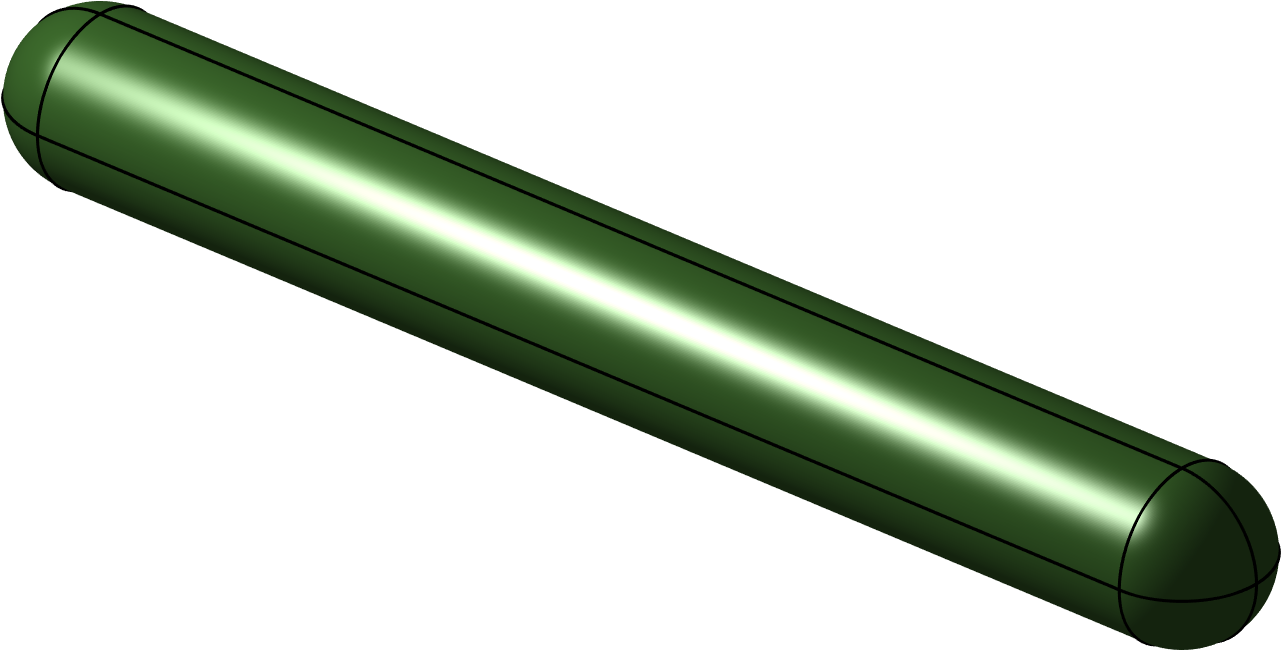
\includegraphics[width=0.7\textwidth]{../../graphics/mockShell}
	\caption[The mock shell]{The mock shell.}
	\label{Fig2:mockShell}
\end{figure}
%
%We shall derive the weak formulation with the most natural choice of the scaling function, namely $s(\zeta) = \zeta$. The weak formulating takes the form: For all $v\in V_1$, find $u_h^N\in V_1$ such that
%\begin{equation*}
%	b_{uc}(u_h^N, v) = \langle g,v\rangle_\Gamma,
%\end{equation*}
%where
%\begin{align}\label{Eq2:infElemntBilinearForm5}
%	b_{uc}(v,u) &= \lim_{\gamma\to\infty}\left(\int_{\Omega_\gamma} (\nabla v \nabla u - k^2 vu)\idiff\Omega - \int_{S_\gamma} v\partial_n u\idiff\Gamma\right),\\
%	\langle g,v\rangle_\Gamma &= \int_\Gamma gv\idiff\Gamma.
%\end{align}
%Here, $S_\gamma$ is the surface where $\zeta = \gamma$ and we can then recover the full domain by letting $\gamma\to\infty$ (which is again dependent on the origin to be placed inside of $\Gamma_{\mathrm{a}}$). For the domain outside the artificial boundary ($\zeta = 1$) we consider trial and test functions of the form
%\begin{equation*}
%	u = \frac{\euler^{\imag r_{\mathrm{a}}k\zeta}}{\zeta^m}\frac{f_m}{r_{\mathrm{a}}^m},\quad v = \frac{\euler^{\imag r_{\mathrm{a}} k\zeta}}{\zeta^n}\frac{f_n}{r_{\mathrm{a}}^n}.
%\end{equation*}
%It is important that these functions are separable. This is obviously the case if $r_{\mathrm{a}}$ is constant, which is the case if $\Gamma_{\mathrm{a}}$ is a sphere. However, for more complex geometries, $r_{\mathrm{a}}$ will depend on the parameters $\xi$ and $\eta$. In order to have separable functions one must then create a series expansion of the exponential function
%\begin{equation*}
%	\euler^{\imag k r_{\mathrm{a}}\zeta} = \sum_{j=1}^\infty \frac{(\imag k r_{\mathrm{a}}\zeta)^j}{j!}
%\end{equation*}
%and take the analytic integration term wise. In the following we will only consider the simple case of $\Gamma_{\mathrm{a}}$ being a sphere (with arbitrary radius). In the general case we have,
%\begin{align*}
%	\nabla v\cdot\nabla u &= \left(\frac{1}{\zeta}\nabla_S v + \vec{a}\pderiv{v}{\zeta}\right)\cdot\left(\frac{1}{\zeta}\nabla_S u + \vec{a}\pderiv{u}{\zeta}\right)\\
%	&= \frac{\euler^{2\imag r_{\mathrm{a}} k\zeta}}{\zeta^{m+n+2}}\nabla_S \left(\frac{f_m}{r_{\mathrm{a}}^m}\right)\cdot\nabla_S \left(\frac{f_n}{r_{\mathrm{a}}^n}\right) +\frac{\euler^{2\imag r_{\mathrm{a}} k\zeta}}{\zeta^{m+n+1}}\left(\imag r_{\mathrm{a}} k - \frac{m}{\zeta}\right)\frac{f_m}{r_{\mathrm{a}}^m}\vec{a}\cdot\nabla_S \left(\frac{f_n}{r_{\mathrm{a}}^n}\right)\\
%	&+ \frac{\euler^{2\imag r_{\mathrm{a}} k\zeta}}{\zeta^{m+n+1}}\left(\imag k - \frac{n}{\zeta}\right)\frac{f_n}{r_{\mathrm{a}}^n}\vec{a}\cdot\nabla_S \left(\frac{f_m}{r_{\mathrm{a}}^m}\right) + \norm{\vec{a}}^2\frac{\euler^{2\imag r_{\mathrm{a}} k\zeta}}{\zeta^{m+n}}\left(\imag r_{\mathrm{a}} k - \frac{n}{\zeta}\right)\left(\imag r_{\mathrm{a}} k - \frac{m}{\zeta}\right)\frac{f_m}{r_{\mathrm{a}}^m} \frac{f_n}{r_{\mathrm{a}}^n}.
%\end{align*}
%and
%\begin{align*}
%	v\partial_n u &= v\nabla u\cdot\vec{n} = v\left(\frac{1}{\zeta}\nabla_S u + \vec{a}\pderiv{u}{\zeta}\right)\cdot\vec{n} = \frac{1}{\zeta}v\nabla_S u\cdot\vec{n} + v\pderiv{u}{\zeta}\vec{a}\cdot\vec{n}\\
%	&= \frac{\euler^{2\imag r_{\mathrm{a}} k\zeta}}{\zeta^{m+n+1}}\frac{f_n}{r_{\mathrm{a}}^n}\nabla_S \left(\frac{f_m}{r_{\mathrm{a}}^m}\right)\cdot\vec{n} + \left(\imag r_{\mathrm{a}} k - \frac{m}{\zeta}\right) \frac{\euler^{2\imag r_{\mathrm{a}} k\zeta}}{\zeta^{m+n}}\frac{f_n}{r_{\mathrm{a}}^n} \frac{f_m}{r_{\mathrm{a}}^m}\vec{a}\cdot\vec{n}.
%\end{align*}
%Consider first the boundary integral at $S_\gamma$
%\begin{align*}
%	\int_{S_\gamma} v\partial_n u\idiff\Gamma &= \int_{\Gamma_{\mathrm{a}}}\frac{\euler^{2\imag k R}}{R^{m+n+1}}\frac{f_n}{r_{\mathrm{a}}^n}\nabla_S \left(\frac{f_m}{r_{\mathrm{a}}^m}\right)\cdot\vec{n} R^2 \kappa\idiff S + \int_{\Gamma_{\mathrm{a}}} \left(\imag r_{\mathrm{a}} k - \frac{m}{R}\right) \frac{\euler^{2\imag k R}}{R^{m+n}}\frac{f_n}{r_{\mathrm{a}}^n} \frac{f_m}{r_{\mathrm{a}}^m} \vec{a}\cdot\vec{n}R^2\kappa\idiff S\\
%	&= \frac{\euler^{2\imag k R}}{R^{m+n-1}}\int_{\Gamma_{\mathrm{a}}}\frac{f_n}{r_{\mathrm{a}}^n}\nabla_S \left(\frac{f_m}{r_{\mathrm{a}}^m}\right)\cdot\vec{n}\kappa\idiff S + \frac{\euler^{2\imag k R}}{R^{m+n-2}}\left(\imag r_{\mathrm{a}} k - \frac{m}{R}\right)\int_{\Gamma_{\mathrm{a}}}  \frac{f_n}{r_{\mathrm{a}}^n} \frac{f_m}{r_{\mathrm{a}}^m}\vec{a}\cdot\vec{n}\kappa\idiff S
%\end{align*}
%As $m+n>1$ all terms of order $\mathcal{O}(\gamma^{-(m+n-1)})$ vanish in the limit $\gamma\to\infty$, such that the integral reduces to
%\begin{equation*}
%	\int_{S_\gamma} v\partial_n u\idiff\Gamma = \imag k\frac{\euler^{2\imag k R}}{R^{m+n-2}}\int_{\Gamma_{\mathrm{a}}} \frac{a_{33}}{\bar{h}_{\upzeta}^2} \frac{f_n}{r_{\mathrm{a}}^n} \frac{f_m}{r_{\mathrm{a}}^m}\idiff S
%\end{equation*}
%where we have used \Cref{Eq2:anRel} and \Cref{Eq2:kapparel}.
%
%Combining all of this into \Cref{Eq2:infElemntBilinearForm5} yields
%\begin{align*}
%	b_{uc}(v,u) = \lim_{\gamma\to\infty}&\left\{J_{mn}\int_1^\gamma \frac{\euler^{2\imag r_{\mathrm{a}} k\zeta}}{\zeta^{m+n}}\idiff\zeta + P_{mn}\int_1^\gamma\frac{\euler^{2\imag r_{\mathrm{a}} k\zeta}}{\zeta^{m+n-1}}\left(\imag r_{\mathrm{a}} k - \frac{m}{\zeta}\right)\idiff\zeta\right.\\
%	 &\left.+ Q_{mn}\int_1^\gamma\frac{\euler^{2\imag r_{\mathrm{a}} k\zeta}}{\zeta^{m+n-1}}\left(\imag r_{\mathrm{a}} k - \frac{n}{\zeta}\right)\idiff\zeta \right.\\
%	&\left. + I_{mn}'\int_1^\gamma\frac{\euler^{2\imag r_{\mathrm{a}} k\zeta}}{\zeta^{m+n}}\left[-(r_{\mathrm{a}} k\zeta)^2 - \imag r_{\mathrm{a}} k\zeta(n + m) + nm\right]\idiff\zeta \right.\\
%	&\left.- I_{mn}\int_1^\gamma\frac{\euler^{2\imag r_{\mathrm{a}} k\zeta}}{\zeta^{m+n}}(k\zeta)^2\idiff\zeta - \imag r_{\mathrm{a}} kI_{mn}'\frac{\euler^{2\imag r_{\mathrm{a}} kR}}{R^{m+n-2}}\right\}
%\end{align*}
%where
%\begin{equation}\label{Eq2:infiniteElementsSurfaceIntegrals5}
%\begin{alignedat}{2}
%	& I_{mn} = \int_{\Gamma_{\mathrm{a}}} \frac{f_m}{r_{\mathrm{a}}^m} \frac{f_n}{r_{\mathrm{a}}^n}\idiff S,\qquad\qquad && I_{mn}' = \int_{\Gamma_{\mathrm{a}}} \frac{a_{33}}{\bar{h}_{\upzeta}^2} \frac{f_m}{r_{\mathrm{a}}^m} \frac{f_n}{r_{\mathrm{a}}^n}\idiff S\\
%	& P_{mn} = \int_{\Gamma_{\mathrm{a}}} \frac{f_m}{r_{\mathrm{a}}^m} \vec{a}\cdot\nabla_S \left(\frac{f_n}{r_{\mathrm{a}}^n}\right)\idiff S, \quad && Q_{mn} = \int_{\Gamma_{\mathrm{a}}}\frac{f_n}{r_{\mathrm{a}}^n}\vec{a}\cdot\nabla_S \left(\frac{f_m}{r_{\mathrm{a}}^m}\right) \idiff S\\
%	& J_{mn} = \int_{\Gamma_{\mathrm{a}}} \nabla_S \left(\frac{f_m}{r_{\mathrm{a}}^m}\right) \cdot\nabla_S \left(\frac{f_n}{r_{\mathrm{a}}^n}\right)\idiff S.
%\end{alignedat}	
%\end{equation}
%In the case of spherical coordinates (where $\Gamma_{\mathrm{a}}$ is the unit sphere) we get $P_{mn}=0$, $Q_{mn} = 0$ and $I_{mn} = I_{mn}'$ such that the bilinear form reduces to the expression in~\cite[p. 93]{Ihlenburg1998fea}. Ihlenburg then notes that the integrals of the form
%\begin{equation*}
%	\int_1^\infty\frac{\euler^{2\imag r_{\mathrm{a}} k\zeta}}{\zeta^n}\idiff\zeta,\quad n\geq 1
%\end{equation*}
%exist and may be computed. Indeed, the \textit{exponential integral} function defined by
%\begin{equation*}
%	E_n(x) = \int_1^\infty \frac{\euler^{-x\zeta}}{\zeta^n}\idiff\zeta
%\end{equation*}
%is implemented in \MATLAB for $n=1$, and using the recursive relation
%\begin{equation*}
%	E_n(x) = \frac{1}{n-1}\left(\euler^{-x} - xE_{n-1}(x)\right),\quad n=2,3,4,\dots
%\end{equation*}
%found in~\cite[p. 229]{Abramovitz1964ham}, we can compute the integrals by
%\begin{equation*}
%	\int_1^\infty\frac{\euler^{2\imag r_{\mathrm{a}} k\zeta}}{\zeta^n}\idiff\zeta = E_n(-2\imag r_{\mathrm{a}} k).
%\end{equation*}
%Also for our case, it thus remains to consider the case $n=m=1$. Consider the limit
%\begin{align*}
%	L &= \lim_{\gamma\to\infty}\left[-\left(r_{\mathrm{a}}^2I_{11}' + I_{11}\right)k^2\int_1^\gamma\euler^{2\imag r_{\mathrm{a}} k\zeta}\idiff\zeta - I_{11}'\imag r_{\mathrm{a}} k\euler^{2\imag r_{\mathrm{a}} kR}\right]\\
%	 &= \lim_{\gamma\to\infty}\left[\frac{\imag k}{2}\left(I_{11} - r_{\mathrm{a}}^2I_{11}'\right)\euler^{2\imag k R} - \frac{\imag k}{2}\left(r_{\mathrm{a}}^2I_{11}' + I_{11}\right)\euler^{2\imag k r_{\mathrm{a}}}\right]
%\end{align*}
%which exists since $I_{11} = r_{\mathrm{a}}^2I_{11}'$. The limit reduces therefore to
%\begin{equation*}
%	L = - \frac{\imag k}{2}\left(r_{\mathrm{a}}^2I_{11}' + I_{11}\right)\euler^{2\imag r_{\mathrm{a}} k}
%\end{equation*}
%The bilinear form is then
%\begin{align*}
%	b_{uc}(v,u) &= J_{mn}E_{m+n} +P_{mn}[\imag r_{\mathrm{a}} k E_{m+n-1} - mE_{m+n}]+Q_{mn}[\imag r_{\mathrm{a}} kE_{m+n-1} - nE_{m+n}]\\
%	 &+ I_{mn}'[-(r_{\mathrm{a}} k)^2E_{m+n-2} - \imag r_{\mathrm{a}} k(n+m)E_{m+n-1} + nm E_{m+n}] - I_{mn}k^2E_{m+n-2}
%\end{align*}
%where $E_{n} = E_{n}(-2\imag r_{\mathrm{a}} k)$. And for the special case $n=m=1$ we get
%\begin{align*}
%	b_{uc}(v,u) &= J_{11}E_{2} +P_{11}[\imag r_{\mathrm{a}} k E_{1} - E_{2}]+Q_{11}[\imag r_{\mathrm{a}} kE_{1} - E_{2}]\\
%	 &+ I_{11}'[- 2\imag r_{\mathrm{a}} kE_{1} + E_{2}] - \frac{\imag k}{2}\left(r_{\mathrm{a}}^2 I_{11}' + I_{11}\right)\euler^{2\imag r_{\mathrm{a}} k}
%\end{align*}
%This will also be the result of PG method if the test functions are not conjugated. This is because all integrals exist as $n+m>3$ in this case.
%
%Let
%\begin{equation*}
%	f_n = \sum_{A\in\vec{\eta}_{\mathrm{a}}} R_A c_{nA},\quad f_m = \sum_{B\in\vec{\eta}_{\mathrm{a}}} R_B d_{mB}
%\end{equation*}
%where we bake $r_{\mathrm{a}}^n$ a,d $r_{\mathrm{a}}^m$ into the coefficients of $c_{nA}$ and $d_{mB}$, respectively.
%
%where $\vec{\eta}_{\mathrm{a}}$ is the set containing the indices of all the basis functions that are non-zero on $\Gamma_{\mathrm{a}}$. As the $b_{uc}$ are linear we then obtain (for $\zeta > 1$)
%\begin{equation*}
%	\sum_{A\in\vec{\eta}_{\mathrm{a}}}\sum_{n=1}^N c_{nA}\left(\sum_{B\in\vec{\eta}_{\mathrm{a}}}\sum_{m=1}^N d_{nA} b_{uc}(R_A, R_B)\right) = 0.
%\end{equation*}
%As the surface integrals in \Cref{Eq2:infiniteElementsSurfaceIntegrals5} will now be independent of the indices $m$ and $n$ we could now define the bilinear form by (for $n+m>1$)
%\begin{align*}
%	b_{uc}(R_A,R_B) &= J_{AB} E_{m+n} +P_{AB} [\imag k E_{m+n-1} - mE_{m+n}]+Q_{AB} [\imag kE_{m+n-1} - nE_{m+n}]\\
%	 &+ I_{AB}'[-k^2E_{m+n-2} - \imag k(n+m)E_{m+n-1} + nm E_{m+n}] - I_{AB} k^2E_{m+n-2}
%\end{align*}
%and for the case $n=m=1$ by
%\begin{align*}
%	b_{uc}(v,u) &= J_{AB}E_{2} +P_{AB}[\imag r_{\mathrm{a}} k E_{1} - E_{2}]+Q_{AB}[\imag r_{\mathrm{a}} kE_{1} - E_{2}]\\
%	 &+ I_{AB}'[- 2\imag r_{\mathrm{a}}kE_{1} + E_{2}] - \frac{\imag k}{2}\left(r_{\mathrm{a}}^2I_{AB}' + I_{AB}\right)\euler^{2\imag k}
%\end{align*}
%where we have redefined the surface integral notations to be
%\begin{alignat*}{2}
%	& I_{AB} = \int_{\Gamma_{\mathrm{a}}} R_A R_B \idiff S,\qquad\qquad && P_{AB} = \int_{\Gamma_{\mathrm{a}}} R_B \vec{a}\cdot\nabla_S R_A\idiff S\\
%	& I_{AB}' = \int_{\Gamma_{\mathrm{a}}} \norm{\vec{a}}^2 R_A R_B\idiff S, \quad && Q_{AB} = \int_{\Gamma_{\mathrm{a}}}R_A\vec{a}\cdot\nabla_S R_B \idiff S\\
%	& J_{AB} = \int_{\Gamma_{\mathrm{a}}} \nabla_S R_B \cdot\nabla_S R_A\idiff S.
%\end{alignat*}
%The infinite elements are thus only contributing whenever we have an element adjacent to the boundary $\Gamma_{\mathrm{a}}$. It is important to note that we now have increased the number of degrees of freedom at the surface $\Gamma_{\mathrm{a}}$ from $|\vec{\eta}_{\mathrm{a}}|$ to $N|\vec{\eta}_{\mathrm{a}}|$. Hence, the method of infinite elements adds a total of $(N-1)|\vec{\eta}_{\mathrm{a}}|$ degrees of freedom. Also note that the surface integrals for $P_{AB}$ and $Q_{AB}$ results in the same set of values. In fact $Q_{AB} = P_{BA}$.  Due to redundancy, we should not evaluate the full 3D NURBS function set at $\zeta=1$ as the 3D NURBS basis functions reduce to a 2D NURBS surface in 3D. Rather, we loop over the surface elements which is then done separate from the main matrix assembly. Thus, the procedure of adding contribution from infinite elements follows the procedure of applying Neumann conditions except that we do not update the load vector $\vec{F}$, rather, we now update the global matrix.
%
%
%
%
%
%
%
%
%
%
%It is also possible to use the complex conjugate of the test functions. In stead of a bilinear form, we then get a sesquilinear form.  The weak formulating then takes the form: For all $v\in V_1$, find $u_h^N\in V_1$ such that
%\begin{equation*}
%	b_c(u_h^N, v) = \langle g,v\rangle_\Gamma,
%\end{equation*}
%where
%\begin{align}\label{Eq2:infElemntBilinearForm6}
%	b_c(v,u) &= \lim_{\gamma\to\infty}\left(\int_{\Omega_\gamma} (\nabla \bar{v} \nabla u - k^2 \bar{v}u)\idiff\Omega - \int_{S_\gamma} \bar{v}\partial_n u\idiff\Gamma\right),\\
%	\langle g,\bar{v}\rangle_\Gamma &= \int_\Gamma g\bar{v}\idiff\Gamma.
%\end{align}
%Again we consider trial and test functions of the form
%\begin{equation*}
%	u = \frac{\euler^{\imag r_{\mathrm{a}} k\zeta}}{\zeta^m}\frac{f_m}{r_{\mathrm{a}}^m},\quad v = \frac{\euler^{\imag r_{\mathrm{a}} k\zeta}}{\zeta^n}\frac{f_n}{r_{\mathrm{a}}^n},\quad
%\end{equation*}
%such that
%\begin{align*}
%	\nabla \bar{v}\cdot\nabla u &= \left(\frac{1}{\zeta}\nabla_S \bar{v} + \vec{a}\pderiv{\bar{v}}{\zeta}\right)\cdot\left(\frac{1}{\zeta}\nabla_S u + \vec{a}\pderiv{u}{\zeta}\right)\\
%	&= \frac{1}{\zeta^{m+n+2}}\nabla_S \left(\frac{f_m}{r_{\mathrm{a}}^m}\right)\cdot\nabla_S \frac{\bar{f}_n}{r_{\mathrm{a}}^n} +\frac{1}{\zeta^{m+n+1}}\left(\imag k - \frac{m}{\zeta}\right)\frac{f_m}{r_{\mathrm{a}}^m}\vec{a}\cdot\nabla_S \frac{\bar{f}_n}{r_{\mathrm{a}}^n}\\
%	&+ \frac{1}{\zeta^{m+n+1}}\left(-\imag k - \frac{n}{\zeta}\right)\frac{\bar{f}_n}{r_{\mathrm{a}}^n}\vec{a}\cdot\nabla_S \left(\frac{f_m}{r_{\mathrm{a}}^m}\right) + \norm{\vec{a}}^2\frac{1}{\zeta^{m+n}}\left(-\imag k - \frac{n}{\zeta}\right)\left(\imag k - \frac{m}{\zeta}\right)\frac{f_m}{r_{\mathrm{a}}^m} \frac{\bar{f}_n}{r_{\mathrm{a}}^n}.
%\end{align*}
%and
%\begin{align*}
%	\bar{v}\partial_n u &= \bar{v}\nabla u\cdot\vec{n} = \bar{v}\left(\frac{1}{\zeta}\nabla_S u + \vec{a}\pderiv{u}{\zeta}\right)\cdot\vec{n} = \frac{1}{\zeta}\bar{v}\nabla_S u\cdot\vec{n} + \bar{v}\pderiv{u}{\zeta}\vec{a}\cdot\vec{n}\\
%	&= \frac{1}{\zeta^{m+n+1}}\frac{\bar{f}_n}{r_{\mathrm{a}}^n}\nabla_S \left(\frac{f_m}{r_{\mathrm{a}}^m}\right)\cdot\vec{n} + \left(\imag k - \frac{m}{\zeta}\right) \frac{1}{\zeta^{m+n}}\frac{\bar{f}_n}{r_{\mathrm{a}}^n} \frac{f_m}{r_{\mathrm{a}}^m}\vec{a}\cdot\vec{n}.
%\end{align*}
%Again we first consider the boundary integral at $S_\gamma$
%\begin{align*}
%	\int_{S_\gamma} \bar{v}\partial_n u\idiff\Gamma &= \int_{\Gamma_{\mathrm{a}}}\frac{1}{R^{m+n+1}}\frac{\bar{f}_n}{r_{\mathrm{a}}^n}\nabla_S \left(\frac{f_m}{r_{\mathrm{a}}^m}\right)\cdot\vec{n} R^2 \kappa\idiff S + \int_{\Gamma_{\mathrm{a}}} \left(\imag k - \frac{m}{R}\right) \frac{1}{R^{m+n}}\frac{\bar{f}_n}{r_{\mathrm{a}}^n} \frac{f_m}{r_{\mathrm{a}}^m} \vec{a}\cdot\vec{n}R^2\kappa\idiff S\\
%	&= \frac{1}{R^{m+n-1}}\int_{\Gamma_{\mathrm{a}}}\frac{\bar{f}_n}{r_{\mathrm{a}}^n}\nabla_S \left(\frac{f_m}{r_{\mathrm{a}}^m}\right)\cdot\vec{n}\kappa\idiff S + \frac{1}{R^{m+n-2}}\left(\imag k - \frac{m}{R}\right)\int_{\Gamma_{\mathrm{a}}}  \frac{\bar{f}_n}{r_{\mathrm{a}}^n} \frac{f_m}{r_{\mathrm{a}}^m}\vec{a}\cdot\vec{n}\kappa\idiff S
%\end{align*}
%As $m+n>1$ all terms of order $\mathcal{O}(\gamma^{-(m+n-1)})$ vanish in the limit $\gamma\to\infty$, such that the integral reduces to
%\begin{equation*}
%	\int_{S_\gamma} v\partial_n u\idiff\Gamma = \imag k\frac{1}{R^{m+n-2}}\int_{\Gamma_{\mathrm{a}}} \frac{a_{33}}{\bar{h}_{\upzeta}^2} \frac{\bar{f}_n}{r_{\mathrm{a}}^n} \frac{f_m}{r_{\mathrm{a}}^m}\idiff S
%\end{equation*}
%Combining all of this into \Cref{Eq2:infElemntBilinearForm6} yields
%\begin{align*}
%	b_c(v,u) = \lim_{\gamma\to\infty}&\left\{J_{mn}\int_1^\gamma \frac{1}{\zeta^{m+n}}\idiff\zeta + P_{mn}\int_1^\gamma\frac{1}{\zeta^{m+n-1}}\left(\imag k - \frac{m}{\zeta}\right)\idiff\zeta\right.\\
%	 &\left.+ Q_{mn}\int_1^\gamma\frac{1}{\zeta^{m+n-1}}\left(-\imag k - \frac{n}{\zeta}\right)\idiff\zeta \right.\\
%	&\left. + I_{mn}'\int_1^\gamma\frac{1}{\zeta^{m+n}}\left[(k\zeta)^2 - \imag k\zeta(n - m) + nm\right]\idiff\zeta \right.\\
%	&\left.- I_{mn}\int_1^\gamma\frac{1}{\zeta^{m+n}}(k\zeta)^2\idiff\zeta - \imag kI_{mn}'\frac{1}{R^{m+n-2}}\right\}
%\end{align*}
%where
%\begin{equation}\label{Eq2:infiniteElementsSurfaceIntegrals6}
%\begin{alignedat}{2}
%	& I_{mn} = \int_{\Gamma_{\mathrm{a}}} \frac{f_m}{r_{\mathrm{a}}^m} \frac{\bar{f}_n}{r_{\mathrm{a}}^n}\idiff S,\qquad\qquad && I_{mn}' = \int_{\Gamma_{\mathrm{a}}} \frac{a_{33}}{\bar{h}_{\upzeta}^2} \frac{f_m}{r_{\mathrm{a}}^m} \frac{\bar{f}_n}{r_{\mathrm{a}}^n}\idiff S\\
%	& P_{mn} = \int_{\Gamma_{\mathrm{a}}} \frac{f_m}{r_{\mathrm{a}}^m} \vec{a}\cdot\nabla_S \frac{\bar{f}_n}{r_{\mathrm{a}}^n}\idiff S, \quad && Q_{mn} = \int_{\Gamma_{\mathrm{a}}}\frac{\bar{f}_n}{r_{\mathrm{a}}^n}\vec{a}\cdot\nabla_S \left(\frac{f_m}{r_{\mathrm{a}}^m}\right) \idiff S\\
%	& J_{mn} = \int_{\Gamma_{\mathrm{a}}} \nabla_S \left(\frac{f_m}{r_{\mathrm{a}}^m}\right) \cdot\nabla_S \frac{\bar{f}_n}{r_{\mathrm{a}}^n}\kappa\idiff S.
%\end{alignedat}	
%\end{equation}
%This time we not only need to consider the case $n=m=1$, but also the cases $n+m=3$. For the case $n+m=3$ we observe that we are depending on the cancellation of the terms involving $\frac{1}{\zeta^{m+n-2}}$. This occurs only if $I_{mn} = I_{mn}'$. Assume this to be the case. We must then consider the the limit (when $n=m=1$)
%\begin{align*}
%	L &= \lim_{\gamma\to\infty}\left[P_{11}\int_1^\gamma \frac{\imag k}{\zeta}\idiff\zeta - Q_{11}\int_1^\gamma \frac{\imag k}{\zeta}\idiff\zeta\right]\\
%	 &= \lim_{\gamma\to\infty}\left[\imag k(P_{11} - Q_{11})\int_1^\gamma \frac{\diff \zeta}{\zeta}\right]
%\end{align*}
%which exists if $P_{11} = Q_{11}$. Again, this only holds for special surfaces $\Gamma_{\mathrm{a}}$, like the unit sphere.  If this is the case, the limit is simply zero.
%
%For $m+n>2$ we simply evaluate the integrals
%\begin{equation*}
%	\int_1^\infty \frac{\diff\zeta}{\zeta^n} = \frac{1}{n-1},\quad n>1.
%\end{equation*}
%The sesquilinear form is then
%\begin{align*}
%	b_c(v,u) &= \frac{J_{mn}}{m+n-1} +P_{mn}\left(\frac{\imag k}{m+n-2} - \frac{m}{m+n-1}\right)+Q_{mn}\left(\frac{-\imag k}{m+n-2} - \frac{n}{m+n-1}\right)\\
%	 &+ I_{mn}'\left(\frac{k^2}{m+n-3} - \frac{\imag k(n-m)}{m+n-2} + \frac{nm}{n+m-1}\right) - I_{mn}\frac{k^2}{m+n-3}
%\end{align*}
%
%Let
%\begin{equation*}
%	\frac{f_n}{r_{\mathrm{a}}^n} = \sum_{A\in\vec{\eta}_{\mathrm{a}}} R_A c_{nA},\quad \frac{f_m}{r_{\mathrm{a}}^m} = \sum_{B\in\vec{\eta}_{\mathrm{a}}} R_B d_{mB}
%\end{equation*}
%where $\vec{\eta}_{\mathrm{a}}$ is the set containing the indices of all the basis functions that are non-zero on $\Gamma_{\mathrm{a}}$. As the $b_{uc}$ are linear we then obtain (for $\zeta > 1$)
%\begin{equation*}
%	\sum_{A\in\vec{\eta}_{\mathrm{a}}}\sum_{n=1}^N \bar{c}_{nA}\left(\sum_{B\in\vec{\eta}_{\mathrm{a}}}\sum_{m=1}^N d_{nA} b_{uc}(R_A, R_B)\right) = 0.
%\end{equation*}
%As the surface integrals in \Cref{Eq2:infiniteElementsSurfaceIntegrals6} will now be independent of the indices $m$ and $n$ we could now define the sesquilinear form by (for $n+m>1$)
%\begin{align*}
%	b_c(R_A,R_B) &= \frac{J_{AB}}{m+n-1} +P_{AB}\left(\frac{\imag k}{m+n-2} - \frac{m}{m+n-1}\right)\\
%	&+Q_{AB}\left(\frac{-\imag k}{m+n-2} - \frac{n}{m+n-1}\right)\\
%	 &+ I_{AB}'\left(\frac{k^2}{m+n-3} - \frac{\imag k(n-m)}{m+n-2} + \frac{nm}{n+m-1}\right) - I_{AB}\frac{k^2}{m+n-3}
%\end{align*}
%We must thus conclude that the extended NURBS coordinate system works best for Petrov--Galerkin methods as there will be no further restriction on the surface $\Gamma_{\mathrm{a}}$. For Bubnov--Galerkin methods the surface $\Gamma_{\mathrm{a}}$ is restricted to surfaces like the unit sphere, which then eliminates the point of introducing the extended NURBS coordinate system in the first place.
%
%The motivation of introducing the extended NURBS coordinate system is to be able to controle the artificial boundary $\Gamma_{\mathrm{a}}$. This allows us to control the size of the fluid domain which would in turn able us to reduce redundant fluid elements. Ihlenburg uses a prolate spheroid as the artificial boundary around his ``Mock shell'' in~\cite{Ihlenburg1998fea}. As the ``Mock shell'' is a convex surface, one could have a uniform thickness of the fluid around the shell by the extended NURBS coordinate system, and thus reducing the fluid computational domain to an ideal size. 

%
\subsection{The cylindrical coordinate system}
\label{Sec2:cylindricalCoordinates}
\tikzsetnextfilename{polarDecomposition_11}
\begin{figure}
	\centering
	\begin{tikzpicture}
	\def\x{1.414213562373095}
	 
	\draw [->](0,1) -- (7,1) node[right] {$x$};
	\draw [->](1,0) -- (1,7) node[above] {$y$};
	
	\draw [-](1,1) -- (4,4);
	
	\draw [dashed] (4,4) node (v1) {} ellipse (2 and 2);
	
	\draw (2,1) arc (0:45:1);
	
	  
	\draw[->] (4,4) -- (4-\x, 4+\x) node (v2) {};
	\draw[->]  (4,4) -- (4,6);
	\draw[->] (4,4) -- (4+\x, 4+\x) node (v3) {};
	\draw[->] (4,4) -- (6,4);
	\draw[->] (4,4) -- (2,4);
	
	\draw[dotted] (v2) -- (4-\x,4);
	\draw[dotted] (v3) -- (4+\x,4);
	
	\node at (2.1,1.5) {$\vartheta$};
	\node at (6.3,4) {$\vec{e}_{\mathrm{x}}$};
	\node at (2-0.5,4) {$-\vec{e}_{\mathrm{x}}$};
	\node at (4,6.3) {$\vec{e}_{\mathrm{y}}$};
	\node at (2.4,5.6) {$\vec{e}_{\upvartheta}$};
	\node at (5.6,5.6) {$\vec{e}_{\mathrm{r}}$};
	
	\node at (2*1.59,2*1.91) {\scriptsize $\sin\vartheta$};
	\node at (4.7,2*1.9) {\scriptsize $\cos\vartheta$};
	
	\node at (2.4,4.6)[rotate=90] {\scriptsize $\cos\vartheta$};
	\node at (6-0.4,4.6)[rotate=90] {\scriptsize $\sin\vartheta$};
	
	\node at (4-\x+0.2,5-0.2) {\scriptsize $\vartheta$};
	\node at (4+0.6,4+0.3) {\scriptsize $\vartheta$};
	
	\draw (4-\x,5) arc (-90:-45:\x-1);
	\draw (4+\x-1,4) arc (0:45:\x-1);
	
	\end{tikzpicture}
	\caption[Unit vectors in polar coordinate system]{Decomposition of the standard unit vectors in the polar coordinate system to the standard unit vectors in the Cartesian coordinate system.}
	\label{Fig2:polarDecomposition}
\end{figure}
The cylindrical coordinate system is simply an extension of the polar coordinate system, which from standard Cartesian coordinates is given by the transformation
\begin{align*}
	x &= r\cos\vartheta\\
	y &= r\sin\vartheta\\
\end{align*}
such that
\begin{align*}
	r &= \sqrt{x^2+y^2}\\
	\vartheta &= \operatorname{atan2}(y,x)
\end{align*}
where
\begin{equation*}
	\operatorname{atan2}(y,x) = \begin{cases}
	\arctan(\frac{y}{x}) & \mbox{if } x > 0\\
	\arctan(\frac{y}{x}) + \PI & \mbox{if } x < 0 \mbox{ and } y \ge 0\\
	\arctan(\frac{y}{x}) - \PI & \mbox{if } x < 0 \mbox{ and } y < 0\\
	\frac{\PI}{2} & \mbox{if } x = 0 \mbox{ and } y > 0\\
	-\frac{\PI}{2} & \mbox{if } x = 0 \mbox{ and } y < 0\\
	\text{undefined} & \mbox{if } x = 0 \mbox{ and } y = 0
	\end{cases}.
\end{equation*}
By this we find
\begin{alignat*}{3}
	\pderiv{r}{x} &= \cos\vartheta,\qquad	&&\pderiv{r}{y} = \sin\vartheta\\
	\pderiv{\vartheta}{x} &= -\frac{1}{r}\sin\vartheta,\qquad	&&\pderiv{\vartheta}{y} = \frac{1}{r}\cos\vartheta.
\end{alignat*}
So for a scalar valued function $\psi$ we get (using the chain rule)
\begin{align}
\label{Eq2:derivativesInPolar}
\begin{split}
	\pderiv{\psi}{x} = \pderiv{\psi}{r}\pderiv{r}{x} + \pderiv{\psi}{\vartheta}\pderiv{\vartheta}{x} = \cos\vartheta\pderiv{\psi}{r} -\frac{1}{r}\sin\vartheta \pderiv{\psi}{\vartheta}\\
	\pderiv{\psi}{y} = \pderiv{\psi}{r}\pderiv{r}{y} + \pderiv{\psi}{\vartheta}\pderiv{\vartheta}{y} = \sin\vartheta\pderiv{\psi}{r} + \frac{1}{r}\cos\vartheta\pderiv{\psi}{\vartheta}
\end{split}
\end{align}
Moreover, by decomposing the standard unit vectors in the polar coordinate system to the standard unit vectors in the Cartesian coordinate system (cf. \Cref{Fig2:polarDecomposition}) we get
\begin{align*}
	\vec{e}_{\mathrm{r}} &= \cos\vartheta\vec{e}_{\mathrm{x}} + \sin\vartheta\vec{e}_{\mathrm{y}}\\
	\vec{e}_{\upvartheta} &= -\sin\vartheta\vec{e}_{\mathrm{x}}+\cos\vartheta\vec{e}_{\mathrm{y}}.
\end{align*}
Hence, for any vector valued function in two dimensions
\begin{equation*}
	\vec{\Psi} = \Psi_{\mathrm{x}}\vec{e}_{\mathrm{x}} + \Psi_{\mathrm{y}}\vec{e}_{\mathrm{y}} = \Psi_{\mathrm{r}}\vec{e}_{\mathrm{r}} + \Psi_{\upvartheta}\vec{e}_{\upvartheta}
\end{equation*}
we get the relations (by comparing each component)
\begin{align}
\label{Eq2:PolarToXfun}
\begin{split}
	\Psi_{\mathrm{x}} &= \Psi_{\mathrm{r}}\cos\vartheta - \Psi_{\upvartheta}\sin\vartheta\\
	\Psi_{\mathrm{y}} &= \Psi_{\mathrm{r}}\sin\vartheta + \Psi_{\upvartheta}\cos\vartheta.
\end{split}
\end{align}
By a corresponding argument, we have
\begin{align}
\label{Eq2:XtoPolar}
\begin{split}
	\vec{e}_{\mathrm{x}} &= \cos\vartheta\vec{e}_{\mathrm{r}} - \sin\vartheta\vec{e}_{\upvartheta}\\
	\vec{e}_{\mathrm{y}} &= \sin\vartheta\vec{e}_{\mathrm{r}}+\cos\vartheta\vec{e}_{\upvartheta}
\end{split}
\end{align}
such that
\begin{align*}
	\Psi_{\mathrm{r}} &= \Psi_{\mathrm{x}}\cos\vartheta + \Psi_{\mathrm{y}}\sin\vartheta\\
	\Psi_{\upvartheta} &= -\Psi_{\mathrm{x}}\sin\vartheta + \Psi_{\mathrm{y}}\cos\vartheta.
\end{align*}
All of these relation also holds for cylindrical coordinates as the $z$ variable is the same for both coordinate systems.

Using \Cref{Eq2:derivativesInPolar}, \Cref{Eq2:PolarToXfun} and \Cref{Eq2:XtoPolar} we get
\begin{align}
	\nabla\psi &= \pderiv{\psi}{x}\vec{e}_{\mathrm{x}} + \pderiv{\psi}{y}\vec{e}_{\mathrm{y}} + \pderiv{\psi}{z}\vec{e}_{\mathrm{z}} = \pderiv{\psi}{r}\vec{e}_{\mathrm{r}}+\frac{1}{r}\pderiv{\psi}{\vartheta}\vec{e}_{\upvartheta}+\pderiv{\psi}{z}\vec{e}_{\mathrm{z}} \label{Eq2:delScalarCyl} \\	
	\nabla^2\psi &= \pderiv[2]{\psi}{x} + \pderiv[2]{\psi}{y} + \pderiv[2]{\psi}{z} = \frac{1}{r}\pderiv{}{r}\left(r\pderiv{\psi}{r}\right) + \frac{1}{r^2}\pderiv[2]{\psi}{\vartheta} +\pderiv[2]{\psi}{z}\\
	\nabla\cdot\vec{\Psi} &= \pderiv{\Psi_{\mathrm{x}}}{x}\ + \pderiv{\Psi_{\mathrm{y}}}{y} + \pderiv{\Psi_{\mathrm{z}}}{z} = \frac{1}{r}\pderiv{(r\Psi_{\mathrm{r}})}{r} + \frac{1}{r}\pderiv{\Psi_{\upvartheta}}{\vartheta}+\pderiv{\Psi_{\mathrm{z}}}{z} \label{Eq2:DelDotVecCyl}\\ 
	\nabla^2\vec{\Psi} &= \left(\nabla^2\Psi_{\mathrm{r}} - \frac{1}{r^2}\Psi_{\mathrm{r}}-\frac{2}{r^2}\pderiv{\Psi_{\upvartheta}}{\vartheta}\right)\vec{e}_{\mathrm{r}} + \left(\nabla^2\Psi_{\upvartheta}-\frac{1}{r^2}\Psi_{\upvartheta} + \frac{2}{r^2}\pderiv{\Psi_{\mathrm{r}}}{\vartheta}\right)\vec{e}_{\upvartheta} + \nabla^2\Psi_{\mathrm{z}}\vec{e}_{\mathrm{z}} \label{Eq2:LapVecPotCyl}
\end{align}
For axisymmetric problems, it is also convenient to write the stress field and the strain field in terms of polar coordinates. Recall that
\begin{equation*}
	\begin{bmatrix}
		\sigma_{11}\\
		\sigma_{22}\\
		\sigma_{33}\\
		\sigma_{23}\\
		\sigma_{13}\\
		\sigma_{12}\\
	\end{bmatrix} = \vec{C}
	\begin{bmatrix}
		\varepsilon_{11}\\
		\varepsilon_{22}\\
		\varepsilon_{33}\\
		2\varepsilon_{23}\\
		2\varepsilon_{13}\\
		2\varepsilon_{12}\\
	\end{bmatrix} = \begin{bmatrix}
		2\mu+\lambda & \lambda & \lambda & 0 & 0 & 0\\
		\lambda & 2\mu+\lambda & \lambda & 0 & 0 & 0\\
		\lambda & \lambda & 2\mu+\lambda & 0 & 0 & 0\\
		0 & 0 & 0 & \mu & 0 & 0\\
		0 & 0 & 0 & 0 & \mu & 0\\
		0 & 0 & 0 & 0 & 0 & \mu
	\end{bmatrix}
	\begin{bmatrix}
		\varepsilon_{11}\\
		\varepsilon_{22}\\
		\varepsilon_{33}\\
		2\varepsilon_{23}\\
		2\varepsilon_{13}\\
		2\varepsilon_{12}\\
	\end{bmatrix}.
\end{equation*}
such that if the stress field is given, we may invert the elasticity matrix to find the strain field. We note that
\begin{equation*}
	\vec{C}^{-1} = \frac{1}{E}\begin{bmatrix}
		1 & -\nu & -\nu & 0 & 0 & 0\\
		-\nu & 1 & -\nu & 0 & 0 & 0\\
		-\nu & -\nu & 1 & 0 & 0 & 0\\
		0 & 0 & 0 & \frac{1}{\mu} & 0 & 0\\
		0 & 0 & 0 & 0 & \frac{1}{\mu} & 0\\
		0 & 0 & 0 & 0 & 0 & \frac{1}{\mu}
	\end{bmatrix}.
\end{equation*}
In~\cite[p. 19]{Gould1994itl} we find the transformation formula for the stress tensor from an arbitrary coordinate system to another. If $\vec{e}_i$ and $\vec{e}_i'$ represents the basis vectors of these two coordinate systems and the stress field is known in the first coordinate system, then the stress field in terms of the second coordinate system is found by
\begin{equation*}
	\sigma_{ij}' = \alpha_{ik}\alpha_{jl}\sigma_{kl}
\end{equation*}
where
\begin{equation*}
	\alpha_{ij} = \cos(\vec{e}_i', \vec{e}_j) = \vec{e}_i'\cdot\vec{e}_j
\end{equation*}
represents the cosine of the angle between the axis corresponding to the vectors $\vec{e}_i$ and $\vec{e}_i'$, respectively. Letting $\vec{e}_1' = \vec{e}_{\mathrm{r}}$, $\vec{e}_2' = \vec{e}_{\mathrm{r}}$ and $\vec{e}_3' = \vec{e}_{\mathrm{z}}$ (the basis vectors in cylindrical coordinates), and $\{\vec{e}_1, \vec{e}_2, \vec{e}_3\}$ the standard basis vectors in Cartesian coordinates, we find (using \Cref{Eq2:XtoPolar})
\begin{equation*}
	[\alpha_{ij}] = \begin{bmatrix}
	\cos\vartheta & \sin\vartheta & 0\\
	-\sin\vartheta & \cos\vartheta & 0\\
	0 & 0 & 1
	\end{bmatrix}.
\end{equation*}
This yields the following relations
\begin{align*}
	\sigma_{\mathrm{rr}} &= \sigma_{11}\cos^2\vartheta + \sigma_{22}\sin^2\vartheta + \sigma_{12}\sin(2\vartheta)\\
	\sigma_{\upvartheta\upvartheta} &= \sigma_{11}\sin^2\vartheta + \sigma_{22}\cos^2\vartheta - \sigma_{12}\sin(2\vartheta)\\
	\sigma_{\mathrm{zz}} &= \sigma_{33}\\
	\sigma_{\upvartheta\mathrm{z}} &= \sigma_{23}\cos\vartheta - \sigma_{13}\sin\vartheta\\
	\sigma_{\mathrm{rz}} &= \sigma_{23}\sin\vartheta + \sigma_{13}\cos\vartheta\\
	\sigma_{\mathrm{r}\upvartheta} &= -\frac{1}{2}\sigma_{11}\sin(2\vartheta) + \frac{1}{2}\sigma_{22}\sin(2\vartheta) + \sigma_{12}\cos(2\vartheta)
\end{align*}
The inverse relations are found to be
\begin{align*}
	\sigma_{11} &= \sigma_{\mathrm{rr}}\cos^2\vartheta + \sigma_{\upvartheta\upvartheta}\sin^2\vartheta - \sigma_{\mathrm{r}\upvartheta}\sin(2\vartheta)\\
	\sigma_{22} &= \sigma_{\mathrm{rr}}\sin^2\vartheta + \sigma_{\upvartheta\upvartheta}\cos^2\vartheta + \sigma_{\mathrm{r}\upvartheta}\sin(2\vartheta)\\
	\sigma_{33} &= \sigma_{\mathrm{zz}}\\
	\sigma_{23} &= \sigma_{\upvartheta\mathrm{z}}\cos\vartheta + \sigma_{\mathrm{rz}}\sin\vartheta\\
	\sigma_{13} &= -\sigma_{\upvartheta\mathrm{z}}\sin\vartheta + \sigma_{\mathrm{rz}}\cos\vartheta\\
	\sigma_{12} &= \frac{1}{2}\sin(2\vartheta)\sigma_{\mathrm{rr}} - \frac{1}{2}\sin(2\vartheta)\sigma_{\upvartheta\upvartheta} - \cos(2\vartheta)\sigma_{\mathrm{r}\upvartheta}.
\end{align*}
Moreover, we have
\begin{equation}\label{Eq2:constitutiveRelationPolar}
	\begin{bmatrix}
		\sigma_{\mathrm{rr}}\\
		\sigma_{\upvartheta\upvartheta}\\
		\sigma_{\mathrm{zz}}\\
		\sigma_{\upvartheta\mathrm{z}}\\
		\sigma_{\mathrm{rz}}\\
		\sigma_{\mathrm{r}\upvartheta}\\
	\end{bmatrix} = \vec{C}
	\begin{bmatrix}
		\varepsilon_{\mathrm{rr}}\\
		\varepsilon_{\upvartheta\upvartheta}\\
		\varepsilon_{\mathrm{zz}}\\
		2\varepsilon_{\upvartheta\mathrm{z}}\\
		2\varepsilon_{\mathrm{rz}}\\
		2\varepsilon_{\mathrm{r}\upvartheta}\\
	\end{bmatrix},
\end{equation}
where (see~\cite{Slaughter2002tlt} for details)
\begin{equation}
\label{Eq2:strainsInPolar}
\begin{split}
	\varepsilon_{\mathrm{rr}} &= \pderiv{u_{\mathrm{r}}}{r}\\
	\varepsilon_{\upvartheta\upvartheta} &= \frac{1}{r}\left(\pderiv{u_{\upvartheta}}{\vartheta} + u_{\mathrm{r}}\right)\\
	\varepsilon_{\mathrm{zz}} &= \pderiv{u_z}{z}\\
	\varepsilon_{\upvartheta\mathrm{z}} &= \frac{1}{2}\left(\pderiv{u_{\upvartheta}}{z} + \frac{1}{r}\pderiv{u_z}{\vartheta}\right)\\
	\varepsilon_{\mathrm{rz}} &= \frac{1}{2}\left(\pderiv{u_{\mathrm{r}}}{z} + \pderiv{u_z}{r}\right)\\
	\varepsilon_{\mathrm{r}\upvartheta} &= \frac{1}{2}\left(\frac{1}{r}\pderiv{u_{\mathrm{r}}}{\vartheta} + \pderiv{u_{\upvartheta}}{r} - \frac{u_{\upvartheta}}{r}\right).
\end{split}
\end{equation}


\subsection{The spherical coordinate system}
\label{Sec2:sphericalCoordinates}
There are several conventions for defining the spherical coordinate system, but we shall here follow the ISO standard (International Organization for Standardization), which is the convention often used in physics. The reason why the mathematical convention of the spherical coordinate system is not used (where the angle $\vartheta$ is preserved in the $xy$-plane as in polar coordinates) is because of the existing literature on the subject of this thesis (in particular~\cite{Ihlenburg1998fea}). The spherical coordinate system is defined by the transformation (from the standard Cartesian coordinates)
\begin{align*}
	x &= r\sin\vartheta\cos\phi\\
	y &= r\sin\vartheta\sin\phi\\
	z &= r\cos\vartheta
\end{align*}
such that
\begin{align*}
	r &= \sqrt{x^2+y^2+z^2}\\
	\vartheta &= \arccos\left(\frac{z}{\sqrt{x^2+y^2+z^2}}\right)\\
	\phi &= \operatorname{atan2}(y,x).
\end{align*}
By this we find
\begin{alignat*}{4}
	\pderiv{r}{x} &= \sin\vartheta\cos\phi,\qquad	&&\pderiv{r}{y} = \sin\vartheta\sin\phi,\qquad	&&\pderiv{r}{z} = \cos\vartheta\\
	\pderiv{\vartheta}{x} &= \frac{1}{r}\cos\vartheta\cos\phi,\qquad	&&\pderiv{\vartheta}{y} = \frac{1}{r}\cos\vartheta\sin\phi,\qquad	&&\pderiv{\vartheta}{z} = -\frac{1}{r}\sin\vartheta\\
	\pderiv{\phi}{x} &= -\frac{1}{r}\frac{\sin\phi}{\sin\vartheta},\qquad	&&\pderiv{\phi}{y} = \frac{1}{r}\frac{\cos\phi}{\sin\vartheta},\qquad	&&\pderiv{\phi}{z} = 0.
\end{alignat*}
So for a scalar valued function $\psi$ we get (using the chain rule)
\begin{align}
\label{Eq2:derivativesInSphericalCoordinates}
\begin{split}
	\pderiv{\psi}{x} &= \pderiv{\psi}{r}\pderiv{r}{x} + \pderiv{\psi}{\phi}\pderiv{\phi}{x} + \pderiv{\psi}{\vartheta}\pderiv{\vartheta}{x} =  \sin\vartheta\cos\phi\pderiv{\psi}{r} - \frac{1}{r}\frac{\sin\phi}{\sin\vartheta}\pderiv{\psi}{\phi} + \frac{1}{r}\cos\vartheta\cos\phi\pderiv{\psi}{\vartheta}\\
	\pderiv{\psi}{y} &= \pderiv{\psi}{r}\pderiv{r}{y} + \frac{1}{r}\frac{\cos\phi}{\sin\vartheta}\pderiv{\psi}{\phi} + \pderiv{\psi}{\vartheta}\pderiv{\vartheta}{y} = \sin\vartheta\cos\phi\pderiv{\psi}{r} + \pderiv{\psi}{\phi}\pderiv{\phi}{y} + \frac{1}{r}\cos\vartheta\sin\phi\pderiv{\psi}{\vartheta}\\
	\pderiv{\psi}{z} &= \pderiv{\psi}{r}\pderiv{r}{z} + \pderiv{\psi}{\phi}\pderiv{\phi}{z} + \pderiv{\psi}{\vartheta}\pderiv{\vartheta}{z} = \cos\vartheta\pderiv{\psi}{r} -\frac{1}{r}\sin\vartheta\pderiv{\psi}{\vartheta}\pderiv{\vartheta}{z}
\end{split}
\end{align}
Moreover, by decomposing the standard unit vectors in the polar coordinate system to the standard unit vectors in the Cartesian coordinate system we get
\begin{align*}
	\vec{e}_{\mathrm{r}} &= \sin\vartheta\cos\phi\vec{e}_{\mathrm{x}} + \sin\vartheta\sin\phi\vec{e}_{\mathrm{y}} + \cos\vartheta\vec{e}_{\mathrm{z}}\\
	\vec{e}_{\upvartheta} &= \cos\vartheta\cos\phi\vec{e}_{\mathrm{x}} + \cos\vartheta\sin\phi\vec{e}_{\mathrm{y}} - \sin\vartheta\vec{e}_{\mathrm{z}}\\
	\vec{e}_{\upphi} &= -\sin\phi\vec{e}_{\mathrm{x}} + \cos\phi\vec{e}_{\mathrm{y}}.
\end{align*}
Hence, for any vector valued function in two dimensions
\begin{equation*}
	\vec{\Psi} = \Psi_{\mathrm{x}}\vec{e}_{\mathrm{x}} + \Psi_{\mathrm{y}}\vec{e}_{\mathrm{y}}  + \Psi_{\mathrm{z}}\vec{e}_{\mathrm{z}} = \Psi_{\mathrm{r}}\vec{e}_{\mathrm{r}} + \Psi_{\upphi}\vec{e}_{\upphi} + \Psi_{\upvartheta}\vec{e}_{\upvartheta}
\end{equation*}
we get the relations (by comparing each component)
\begin{align}
\label{Eq2:SphericalToXfun}
\begin{split}
	\Psi_{\mathrm{x}} &= \Psi_{\mathrm{r}}\sin\vartheta\cos\phi + \Psi_{\upvartheta}\cos\vartheta\cos\phi - \Psi_{\upphi}\sin\phi\\
	\Psi_{\mathrm{y}} &= \Psi_{\mathrm{r}}\sin\vartheta\sin\phi + \Psi_{\upvartheta}\cos\vartheta\sin\phi - \Psi_{\upphi}\cos\phi\\
	\Psi_{\mathrm{z}} &= \Psi_{\mathrm{r}}\cos\vartheta - \Psi_{\upvartheta}\sin\vartheta.
\end{split}
\end{align}
By a corresponding argument, we have
\begin{align}
\label{Eq2:XtoSpherical}
\begin{split}
	\vec{e}_{\mathrm{x}} &= \sin\vartheta\cos\phi\vec{e}_{\mathrm{r}} + \cos\vartheta\cos\phi\vec{e}_{\upvartheta} - \sin\phi\vec{e}_{\upphi}\\
	\vec{e}_{\mathrm{y}} &= \sin\vartheta\sin\phi\vec{e}_{\mathrm{r}} + \cos\vartheta\sin\phi\vec{e}_{\upvartheta} + \cos\phi\vec{e}_{\upphi}\\
	\vec{e}_{\mathrm{z}} &= \cos\vartheta\vec{e}_{\mathrm{r}} - \sin\vartheta\vec{e}_{\upvartheta}.
\end{split}
\end{align}
such that
\begin{align*}
\begin{split}
	\Psi_{\mathrm{r}} &= \Psi_{\mathrm{x}}\sin\vartheta\cos\phi + \Psi_{\mathrm{y}}\sin\vartheta\sin\phi + \Psi_{\mathrm{z}}\cos\vartheta\\
	\Psi_{\upvartheta} &= \Psi_{\mathrm{x}}\cos\vartheta\cos\phi + \Psi_{\mathrm{y}}\cos\vartheta\sin\phi - \Psi_{\mathrm{z}}\sin\vartheta\\
	\Psi_{\upphi} &= - \Psi_{\mathrm{x}}\sin\phi + \Psi_{\mathrm{y}}\cos\phi.
\end{split}
\end{align*}
Using \Cref{Eq2:derivativesInSphericalCoordinates}, \Cref{Eq2:SphericalToXfun} and \Cref{Eq2:XtoSpherical} we get
\begin{align}
	\nabla\psi &= \pderiv{\psi}{x}\vec{e}_{\mathrm{x}} + \pderiv{\psi}{y}\vec{e}_{\mathrm{y}} + \pderiv{\psi}{z}\vec{e}_{\mathrm{z}} = \pderiv{\psi}{r}\vec{e}_{\mathrm{r}}+\frac{1}{r}\pderiv{\psi}{\vartheta}\vec{e}_{\upvartheta}+\frac{1}{r\sin\vartheta}\pderiv{\psi}{\phi}\vec{e}_{\upphi} \label{Eq2:delScalarSpherical} \\	
	\nabla^2\psi &= \pderiv[2]{\psi}{x} + \pderiv[2]{\psi}{y} + \pderiv[2]{\psi}{z}\\ 
	&= \frac{1}{r^2}\pderiv{}{r}\left(r^2\pderiv{\psi}{r}\right) + \frac{1}{r^2\sin\vartheta}\pderiv{}{\vartheta}\left(\sin\vartheta\pderiv{\psi}{\vartheta}\right) +\frac{1}{r^2\sin^2\vartheta}\pderiv[2]{\psi}{\phi}\\
	\nabla\cdot\vec{\Psi} &= \pderiv{\Psi_{\mathrm{x}}}{x}\ + \pderiv{\Psi_{\mathrm{y}}}{y} + \pderiv{\Psi_{\mathrm{z}}}{z} = \frac{1}{r^2}\pderiv{(r^2\Psi_{\mathrm{r}})}{r} + \frac{1}{r\sin\vartheta}\pderiv{(\Psi_{\upvartheta}\sin\vartheta)}{\vartheta}+\frac{1}{r\sin\vartheta}\pderiv{\Psi_{\upphi}}{\phi} \label{Eq2:DelDotVecSpherical} \\ 
	\nabla^2\vec{\Psi} &= \left(\nabla^2\Psi_{\mathrm{r}} - \frac{2}{r^2}\Psi_{\mathrm{r}}-\frac{2}{r^2\sin\vartheta}\pderiv{(\Psi_{\upvartheta}\sin\vartheta)}{\vartheta} -\frac{2}{r^2\sin\vartheta}\pderiv{\Psi_{\upphi}}{\phi}\right)\vec{e}_{\mathrm{r}} \\
	&+ \left(\nabla^2\Psi_{\upvartheta}-\frac{1}{r^2\sin^2\vartheta}\Psi_{\upvartheta} + \frac{2}{r^2}\pderiv{\Psi_{\mathrm{r}}}{\vartheta} -\frac{2\cos\vartheta}{r^2\sin^2\vartheta}\pderiv{\Psi_{\upphi}}{\phi}\right)\vec{e}_{\upvartheta} \\
	&+ \left(\nabla^2\Psi_{\upphi} - \frac{1}{r^2\sin^2\vartheta}\Psi_{\upphi} + \frac{2}{r^2\sin\vartheta}\pderiv{\Psi_{\mathrm{r}}}{\phi}+\frac{2\cos\vartheta}{r^2\sin^2\vartheta}\pderiv{\Psi_{\upvartheta}}{\phi}\right)\vec{e}_{\upphi} \label{Eq2:LapVecPotSpherical}
\end{align}
We may also for the spherical coordinates find the relation between the stress fields as we did for the cylindrical coordinates in \Cref{Sec2:cylindricalCoordinates}. In spherical coordinates we get
\begin{equation*}
	[\alpha_{ij}] = \begin{bmatrix}
	\sin\vartheta\cos\phi & \sin\vartheta\sin\phi & \cos\vartheta\\
	\cos\vartheta\cos\phi & \cos\vartheta\sin\phi & -\sin\vartheta\\
	-\sin\phi & \cos\phi & 0
	\end{bmatrix}.
\end{equation*}
Which yields the relation
\begin{equation*}
	\begin{bmatrix}
		\sigma_{\mathrm{rr}}\\
		\sigma_{\upvartheta\upvartheta}\\
		\sigma_{\upphi\upphi}\\
		\sigma_{\upvartheta\upphi}\\
		\sigma_{\mathrm{r}\upphi}\\
		\sigma_{\mathrm{r}\upvartheta}
	\end{bmatrix} = \vec{D}
	\begin{bmatrix}
		\sigma_{11}\\
		\sigma_{22}\\
		\sigma_{33}\\
		\sigma_{23}\\
		\sigma_{13}\\
		\sigma_{12}
	\end{bmatrix}
\end{equation*}
where

\begin{equation*}\resizebox{\linewidth}{!}{$
	\vec{D} =\begin{bmatrix}
	 \sin^2\vartheta\cos^2\phi&\sin^2\vartheta\sin^2\phi&\cos^2\vartheta&\sin2\vartheta\sin\phi&\sin2\vartheta\cos\phi&\sin^2\vartheta\sin2\phi\\ 
	 \cos^2\vartheta\cos^2\phi&\cos^2\vartheta\sin^2\phi&\sin^2\vartheta&-\sin2\vartheta\sin\phi&-\sin2\vartheta\cos\phi&\cos^2\vartheta\sin2\phi\\ 
	 \sin^2\phi&\cos^2\phi&0&0&0&-\sin2\phi\\ 
	 -\frac12\cos\vartheta\sin2\phi&\frac12\cos\vartheta\sin2\phi&0&-\sin\vartheta\cos\phi&\sin\vartheta\sin\phi&\cos\vartheta\cos2\phi\\ 
	 -\frac12\sin\vartheta\sin2\phi&\frac12\sin\vartheta\sin2\phi&0&\cos\vartheta\cos\phi&-\cos\vartheta\sin\phi&\sin\vartheta\cos2\phi\\ 
	 \frac12\sin2\vartheta\cos^2\phi&\frac12\sin2\vartheta\sin^2\phi&-\frac12\sin2\vartheta&\cos2\vartheta\sin\phi&\cos2\vartheta\cos\phi&\frac12\sin2\vartheta\sin2\phi
	\end{bmatrix}$}
\end{equation*}

The inverse relation is found by inverting the matrix $\vec{D}$.

\begin{equation*}\resizebox{\linewidth}{!}{$
	\vec{D}^{-1} =\begin{bmatrix}
	 \sin^2\vartheta\cos^2\phi & \cos^2\vartheta\cos^2\phi & \sin^2\phi & -\cos\vartheta\sin2\phi & -\sin\vartheta\sin2\phi & \sin2\vartheta\cos^2\phi \\
	 \sin^2\vartheta\sin^2\phi & \cos^2\vartheta\sin^2\phi & \cos^2\phi & \cos\vartheta\sin2\phi & \sin\vartheta\sin2\phi & \sin2\vartheta\sin^2\phi\\
	 \cos^2\vartheta & \sin^2\vartheta & 0 & 0 & 0 & -\sin2\vartheta\\
	 \frac12\sin2\vartheta\sin\phi & -\frac12\sin2\vartheta\sin\phi & 0 & -\sin\vartheta\cos\phi & \cos\vartheta\cos\phi & \sin\phi\cos2\vartheta\\
	 -\sin\vartheta\sin2\phi & -\frac12\sin2\vartheta\cos\phi & 0 & \sin\vartheta\sin\phi & -\cos\vartheta\sin\phi & \cos2\vartheta\cos\phi\\
	 \frac12\sin^2\vartheta\sin2\phi & \frac12\cos^2\vartheta\sin2\phi &-\frac12\sin2\phi & \cos\vartheta\cos2\phi & \cos2\phi\sin\vartheta &\frac12\sin2\vartheta\sin2\phi
	\end{bmatrix}$}
\end{equation*}


Moreover, we have
\begin{equation}
\label{Eq2:constitutiveRelationSpherical}
	\begin{bmatrix}
		\sigma_{\mathrm{rr}}\\
		\sigma_{\upvartheta\upvartheta}\\
		\sigma_{\upphi\upphi}\\
		\sigma_{\upvartheta \upphi}\\
		\sigma_{\mathrm{r} \upphi}\\
		\sigma_{\mathrm{r}\upvartheta}\\
	\end{bmatrix} = \vec{C}
	\begin{bmatrix}
		\varepsilon_{\mathrm{rr}}\\
		\varepsilon_{\upvartheta\upvartheta}\\
		\varepsilon_{\upphi\upphi}\\
		2\varepsilon_{\vartheta \phi}\\
		2\varepsilon_{r \phi}\\
		2\varepsilon_{\mathrm{r}\upvartheta}\\
	\end{bmatrix},
\end{equation}
where (see~\cite{Slaughter2002tlt} for details)
\begin{equation}
\label{Eq2:strainsInSpherical}
\begin{split}
	\varepsilon_{\mathrm{rr}} &= \pderiv{u_{\mathrm{r}}}{r}\\
	\varepsilon_{\upvartheta\upvartheta} &= \frac{1}{r}\left(\pderiv{u_{\upvartheta}}{\vartheta} + u_{\mathrm{r}}\right)\\
	\varepsilon_{\upphi\upphi} &= \frac{1}{r\sin\vartheta}\left(\pderiv{u_{\phi}}{\phi} + u_{\mathrm{r}}\sin\vartheta + u_{\upvartheta}\cos\vartheta\right)\\
	\varepsilon_{\upvartheta\upphi} &= \frac{1}{2r}\left(\frac{1}{\sin\vartheta}\pderiv{u_{\upvartheta}}{\phi} + \pderiv{u_{\upphi}}{\vartheta} - u_{\upphi}\cot\vartheta\right)\\
	\varepsilon_{\mathrm{r}\upphi} &= \frac{1}{2}\left(\frac{1}{r\sin\vartheta}\pderiv{u_{\mathrm{r}}}{\phi} + \pderiv{u_{\upphi}}{r} - \frac{u_{\upphi}}{r}\right)\\
	\varepsilon_{\mathrm{r}\upvartheta} &= \frac{1}{2}\left(\frac{1}{r}\pderiv{u_{\mathrm{r}}}{\vartheta} + \pderiv{u_{\upvartheta}}{r} - \frac{u_{\upvartheta}}{r}\right).
\end{split}
\end{equation}

\subsection{The prolate spheroidal coordinate system}
\label{Sec2:prolateSphericalCoordinateSystem}
The prolate spheroidal coordinate system is an extension of the spherical coordinate system. It is defined by the relations
\begin{align*}
	x &= \sqrt{r^2 - f^2}\sin\vartheta\cos\phi\\
	y &= \sqrt{r^2 - f^2}\sin\vartheta\sin\phi\\
	z &= r\cos\vartheta
\end{align*}
with foci located at $z = \pm f$. Note that we define $r\geq f$ such that the coordinate system reduces to the spherical coordinate system when $f=0$. Using this condition, we may establish the following inverse formulas
\begin{align}\label{Eq2:XtoProl}
\begin{split}
	r &= \frac{1}{\sqrt{2}}\sqrt{T_f + \sqrt{T_f^2-4f^2z^2}}\\
	\vartheta &= \arccos\left(\frac{\sqrt{2}z}{\sqrt{T_f + \sqrt{T_f^2-4f^2z^2}}}\right)\\
	\phi &= \operatorname{atan2}(y,x).
\end{split}
\end{align}
where $T_f = T_f(x,y,z) = x^2+y^2+z^2+f^2$.

The derivatives are found to be
\begin{equation}\label{Eq2:dXdProlateSphericalCoordinates}
\begin{alignedat}{4}
	\pderiv{x}{r} &= \frac{r\sin\vartheta\cos\phi}{\sqrt{r^2-f^2}},\qquad	&&\pderiv{y}{r} = \frac{r\sin\vartheta\sin\phi}{\sqrt{r^2-f^2}},\qquad	&&\pderiv{z}{r} = \cos\vartheta\\
	\pderiv{x}{\vartheta} &=\sqrt{r^2-f^2}\cos\vartheta\cos\phi,\qquad	&&\pderiv{y}{\vartheta} = \sqrt{r^2-f^2}\cos\vartheta\sin\phi,\qquad	&&\pderiv{z}{\vartheta} = -r\sin\vartheta\\
	\pderiv{x}{\phi} &= -\sqrt{r^2-f^2}\sin\vartheta\sin\phi,\qquad	&&\pderiv{y}{\phi} = \sqrt{r^2-f^2}\sin\vartheta\cos\phi,\qquad	&&\pderiv{z}{\phi} =0.
\end{alignedat}
\end{equation}
and
\begin{equation}\label{Eq2:dProlateSphericalCoordinatesdX}
\begin{alignedat}{4}
	\pderiv{r}{x} &= \frac{xr}{2r^2-T_f},\qquad	&&\pderiv{r}{y} = \frac{yr}{2r^2-T_f},\qquad	&&\pderiv{r}{z} = \frac{z}{r}\frac{r^2-f^2}{2r^2-T_f}\\
	\pderiv{\vartheta}{x} &= \frac{xz}{r\sin\vartheta (2r^2-T_f)},\qquad	&&\pderiv{\vartheta}{y} = \frac{yz}{r\sin\vartheta (2r^2-T_f)},\qquad	&&\pderiv{\vartheta}{z} = \frac{1}{r\sin\vartheta}\left(\frac{z^2}{r^2}\frac{r^2-f^2}{2r^2-T_f}-1\right)\\
	\pderiv{\phi}{x} &= -\frac{y}{x^2+y^2},\qquad	&&\pderiv{\phi}{y} = \frac{x}{x^2+y^2},\qquad	&&\pderiv{\phi}{z} = 0.
\end{alignedat}
\end{equation}

Using \Cref{Eq2:ScalingLengths} we have
\begin{align*}
	h_{\mathrm{r}} &= \sqrt{\frac{r^2-f^2\cos^2\vartheta}{r^2-f^2}}\\
	h_{\upvartheta} &= \sqrt{r^2-f^2\cos^2\vartheta}\\
	h_{\upphi} &= \sqrt{r^2-f^2}\sin\vartheta	
\end{align*}
As the prolate spheroidal coordinate system is an orthogonal coordinate system, the general nabla operator developed in \Cref{Sec2:general3DcoordinateSystem} reduces to
\begin{equation*}
	\nabla = \frac{\vec{e}_{\mathrm{r}}}{h_{\mathrm{r}}} \pderiv{}{r} + \frac{\vec{e}_{\upvartheta}}{h_{\upvartheta}} \pderiv{}{\vartheta} + \frac{\vec{e}_{\upphi}}{h_{\upphi}} \pderiv{}{\phi}
\end{equation*}
The determinant of the jacobian in \Cref{Eq2:NURBSjacobian} may now be written as
\begin{equation*}
	J_1 = h_{\mathrm{r}} h_{\upvartheta} h_{\upphi} = \left(r^2-f^2\cos^2\vartheta\right)\sin\vartheta
\end{equation*}
The surface Jacobian at a given (constant) $r=\hat{r}$ is
\begin{equation*}
	J_S = h_{\upvartheta} h_{\upphi} = \sqrt{r^2-f^2\cos^2\vartheta}\sqrt{r^2-f^2}\sin\vartheta	.
\end{equation*}
Note that 
\begin{equation*}
	\lim_{\hat{r}\to\infty}J_S = \hat{r}^2\sin\vartheta.
\end{equation*}
That is, in the limit $\hat{r}\to\infty$ the surface Jacobian of the prolate spheroidal coordinate system is the same as the surface Jacobian of the spherical coordinate system.

